%%%%%%%%%%%%%%%%%%%%%%%%%%%%%%%%%%%%%%%%%
% Beamer Presentation
% LaTeX Template
% Version 1.0 (10/11/12)
%
% This template has been downloaded from:
% http://www.LaTeXTemplates.com
%
% License:
% CC BY-NC-SA 3.0 (http://creativecommons.org/licenses/by-nc-sa/3.0/)
%
%%%%%%%%%%%%%%%%%%%%%%%%%%%%%%%%%%%%%%%%%

%-------------------------------------------------------------------------------
%	PACKAGES AND THEMES
%-------------------------------------------------------------------------------

\documentclass{beamer}
\usepackage{xcolor}
\usepackage{graphicx}
\usepackage{tikz}
\usepackage{listings}
\usepackage{multicol}

\DeclareMathOperator{\diag}{diag}

\definecolor{applegreen}{rgb}{0.55, 0.71, 0.0}
\definecolor{blue(ncs)}{rgb}{0.0, 0.45, 0.60}
\definecolor{burgundy}{rgb}{0.5, 0.0, 0.13}

\definecolor{cadet}{rgb}{0.33, 0.41, 0.47}
\definecolor{airforceblue}{rgb}{0.36, 0.54, 0.66}

\mode<presentation> {

\usetheme{CambridgeUS}

\usecolortheme{wolverine}

\definecolor{gold}{HTML}{D4A017}
\definecolor{darkgold}{HTML}{B7950B}

\setbeamercolor{palette primary}{bg=cadet,fg=white}
\setbeamercolor{palette secondary}{bg=airforceblue,fg=white}
\setbeamercolor{palette tertiary}{bg=black,fg=white}
\setbeamercolor{palette quaternary}{bg=cadet,fg=white}

\setbeamercolor{frametitle}{bg=airforceblue,fg=white}

\setbeamercolor{section number projected}{bg=black,fg=cadet}
\setbeamercolor{item}{fg=black,bg=cadet}

\setbeamertemplate{page number in head/foot}[framenumber]

\lstset{basicstyle=\ttfamily\footnotesize,breaklines=true}
}



\lstdefinestyle{colouredC}{ 
  commentstyle=\color[gray]{0.4},
  keywordstyle=\bfseries,
  keywordstyle=[2]\color[rgb]{0.75, 0, 0},
  keywordstyle=[3]\color[rgb]{0, 0.5, 0},
  keywordstyle=[4]\color[rgb]{0, 0.5, 0},
  keywordstyle=[5]\color[rgb]{0, 0, 0.75},
  numberstyle=\tiny\color{mGray},
  stringstyle=\color[rgb]{0, 0, 0.5},
  basicstyle=\ttfamily,
  language=C,
  morekeywords=[3]{CeedInt, CeedScalar},
}

\lstdefinestyle{boxedC}{
  style=colouredC,
  numbers=left,
  firstnumber=auto,
  numberblanklines=true,
  frame=trbL,
  numberstyle=\tiny,
  frame=leftline,
  numbersep=7pt,
  framesep=5pt,
  framerule=10pt,
  xleftmargin=15pt,
  backgroundcolor=\color[gray]{0.97},
  rulecolor=\color[gray]{0.90}%
}

\usepackage{graphicx} % Allows including images
\usepackage{booktabs} % Allows the use of \toprule, \midrule and \bottomrule in tables

\newcommand{\mycomment}[1]{}

%----------------------------------------------------------------------------------------
%	TITLE PAGE
%----------------------------------------------------------------------------------------

\title[Ratel]{Ratel - Solid Mechanics for the Exascale Era
} % The short title appears at the bottom of every slide, the full title is only on the title page

\author{Jeremy L Thompson} % Your name
\institute[CU Boulder] % Your institution as it will appear on the bottom of every slide, may be shorthand to save space
{University of Colorado Boulder \\ % Your institution for the title page
\medskip
\textit{jeremy@jeremylt.org}\\ % Your email address
\textit{Website/CV: \href{https://jeremylt.org}{https://jeremylt.org}}
}
\date{6 August 2025} % Date, can be changed to a custom date

\begin{document}

\begin{frame}
\titlepage % Print the title page as the first slide
\end{frame}

%------------------------------------------------

\begin{frame}
\frametitle{Overview} % Table of contents slide, comment this block out to remove it
\tableofcontents % Throughout your presentation, if you choose to use \section{} and \subsection{} commands, these will automatically be printed on this slide as an overview of your presentation
\end{frame}

%-------------------------------------------------------------------------------
\section{libCEED}
%-------------------------------------------------------------------------------

\begin{frame}
\begin{center}
\frametitle{Top 500}

\begin{table}[ht!]
\begin{center}
\begin{tabular}{l r r}
  \toprule
  Machine  &  HPL  &  HPCG  \\
  \toprule
  El Capitan &  1,742.00 PFLOPs  &  17.41 PFLOPS  \\
  Fugaku     &    442.01 PFLOPs  &  16.00 PFLOPs  \\
  Frontier   &  1,353.00 PFLOPs  &  14.05 PFLOPs  \\
  Aurora     &  1,012.00 PFLOPs  &   5.61 PFLOPs  \\
  LUMI       &    379.70 PFLOPs  &   4.59 PFLOPs  \\
  \bottomrule
\end{tabular}
\end{center}
\end{table}
{\small Top 500 Machines for HPCG with HPL peak FLOPs}\\

~\\

HPCG closer to representative FLOPs for simulations\\

~\\

Difficult to realize peak FLOPs with CG on modern machines

\end{center}
\end{frame}

%------------------------------------------------

\begin{frame}
\begin{center}
\frametitle{Modern Hardware}

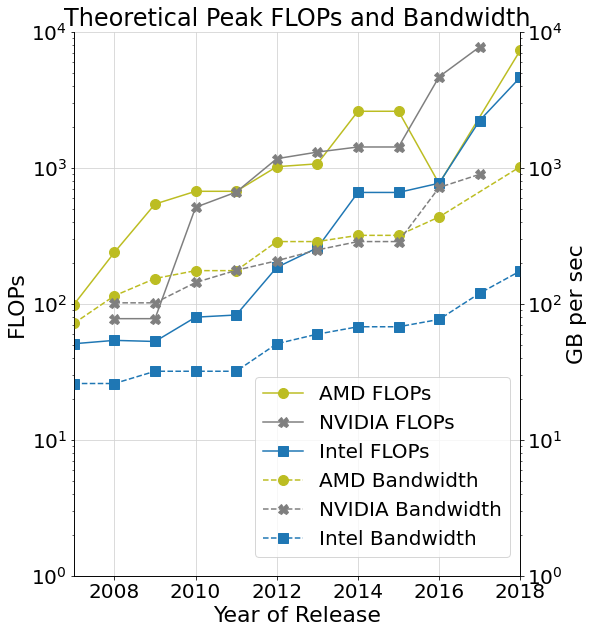
\includegraphics[height=5.5cm]{peakFlopsAndBandwidth_tall.png}
\hspace{1cm}
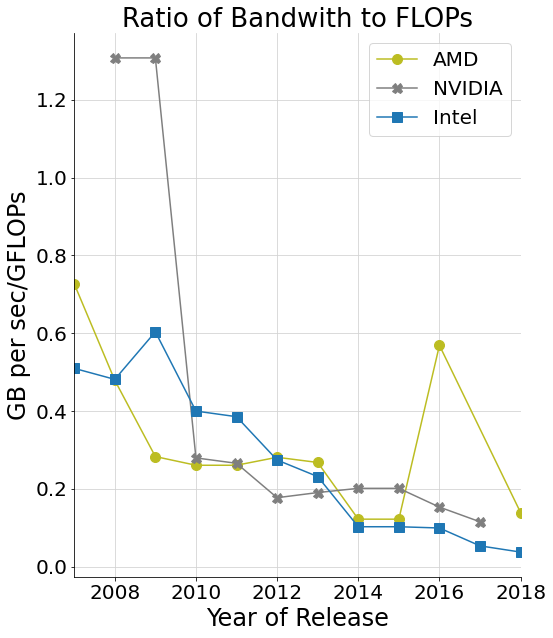
\includegraphics[height=5.5cm]{peakRatio_tall.png}

Memory bandwidth is improving slower than FLOPs\\

~\\

Mirrors difference between Top 500 HPL vs HPCG benchmarks\\

\end{center}
\end{frame}

%------------------------------------------------

\begin{frame}
\begin{center}
\frametitle{Benefits of Matrix-Free}

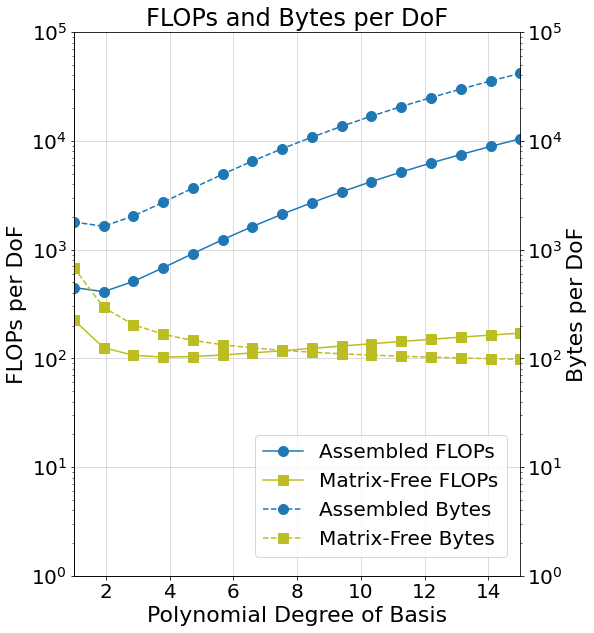
\includegraphics[height=5.5cm]{assembledVsMatrixFree_tall}
\hspace{1cm}
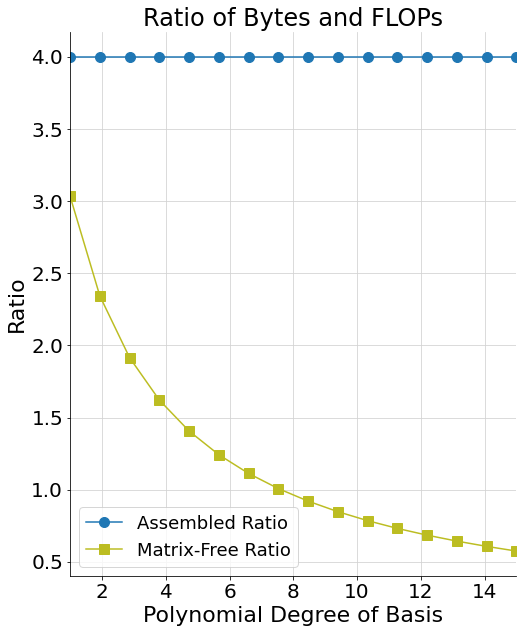
\includegraphics[height=5.5cm]{assembledVsMatrixFreeBalance_tall}

{\small Requirements for matrix-vector product with sparse matrix vs matrix-free\\ for screened Poisson $\nabla^2 u - \alpha^2 u = f$ in 3D}\\

{\bf Matrix-free representations using tensor product bases\\better match modern hardware}

\end{center}
\end{frame}

%------------------------------------------------

\begin{frame}
\frametitle{libCEED Team}

\begin{center}
\includegraphics[height=2.75cm]{libCEEDlogo.png}
\end{center}

{\flushleft

libCEED Repo: \href{https://github.com/CEED/libCEED}{https://github.com/CEED/libCEED}\\

~\\
Developers: Ahmad Abdelfattah, Zach R. Atkins, Valeria Barra,\\
\hspace{19mm} Natalie Beams, Jed Brown, Jean-Sylvain Camier,\\
\hspace{19mm} Veselin Dobrev, Yohann Dudouit, Leila Ghaffari,\\
\hspace{19mm} Sebastian Grimberg, Tzanio Kolev, David Medina,\\
\hspace{19mm} Will Paznel, Thilina Ratnayaka, Rezgar Shakeri,\\
\hspace{19mm} Stan Tomov, James Wright III, Jeremy L Thompson\\

~\\

}

\end{frame}

%------------------------------------------------

\begin{frame}
\begin{center}
\frametitle{Matrix-Free Operators with libCEED}

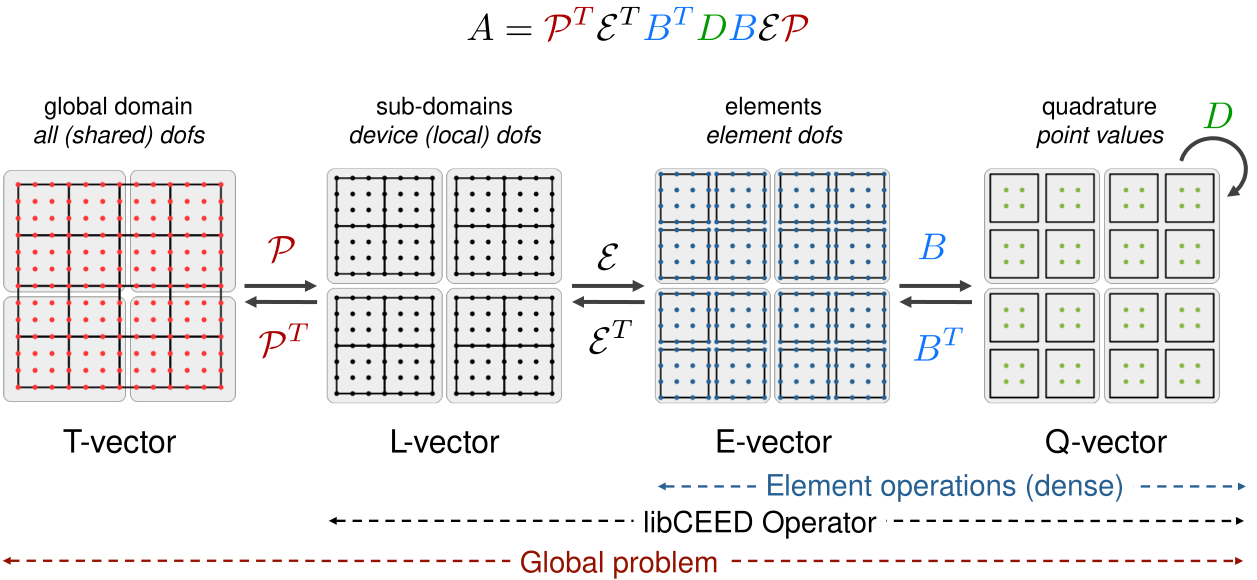
\includegraphics[height=5.0cm]{libCEEDAPI.png}

~\\

libCEED provides arbitrary order matrix-free operator evaluation\\

\end{center}
\end{frame}

%------------------------------------------------

\begin{frame}
\begin{center}
\frametitle{Performance Portability from libCEED}

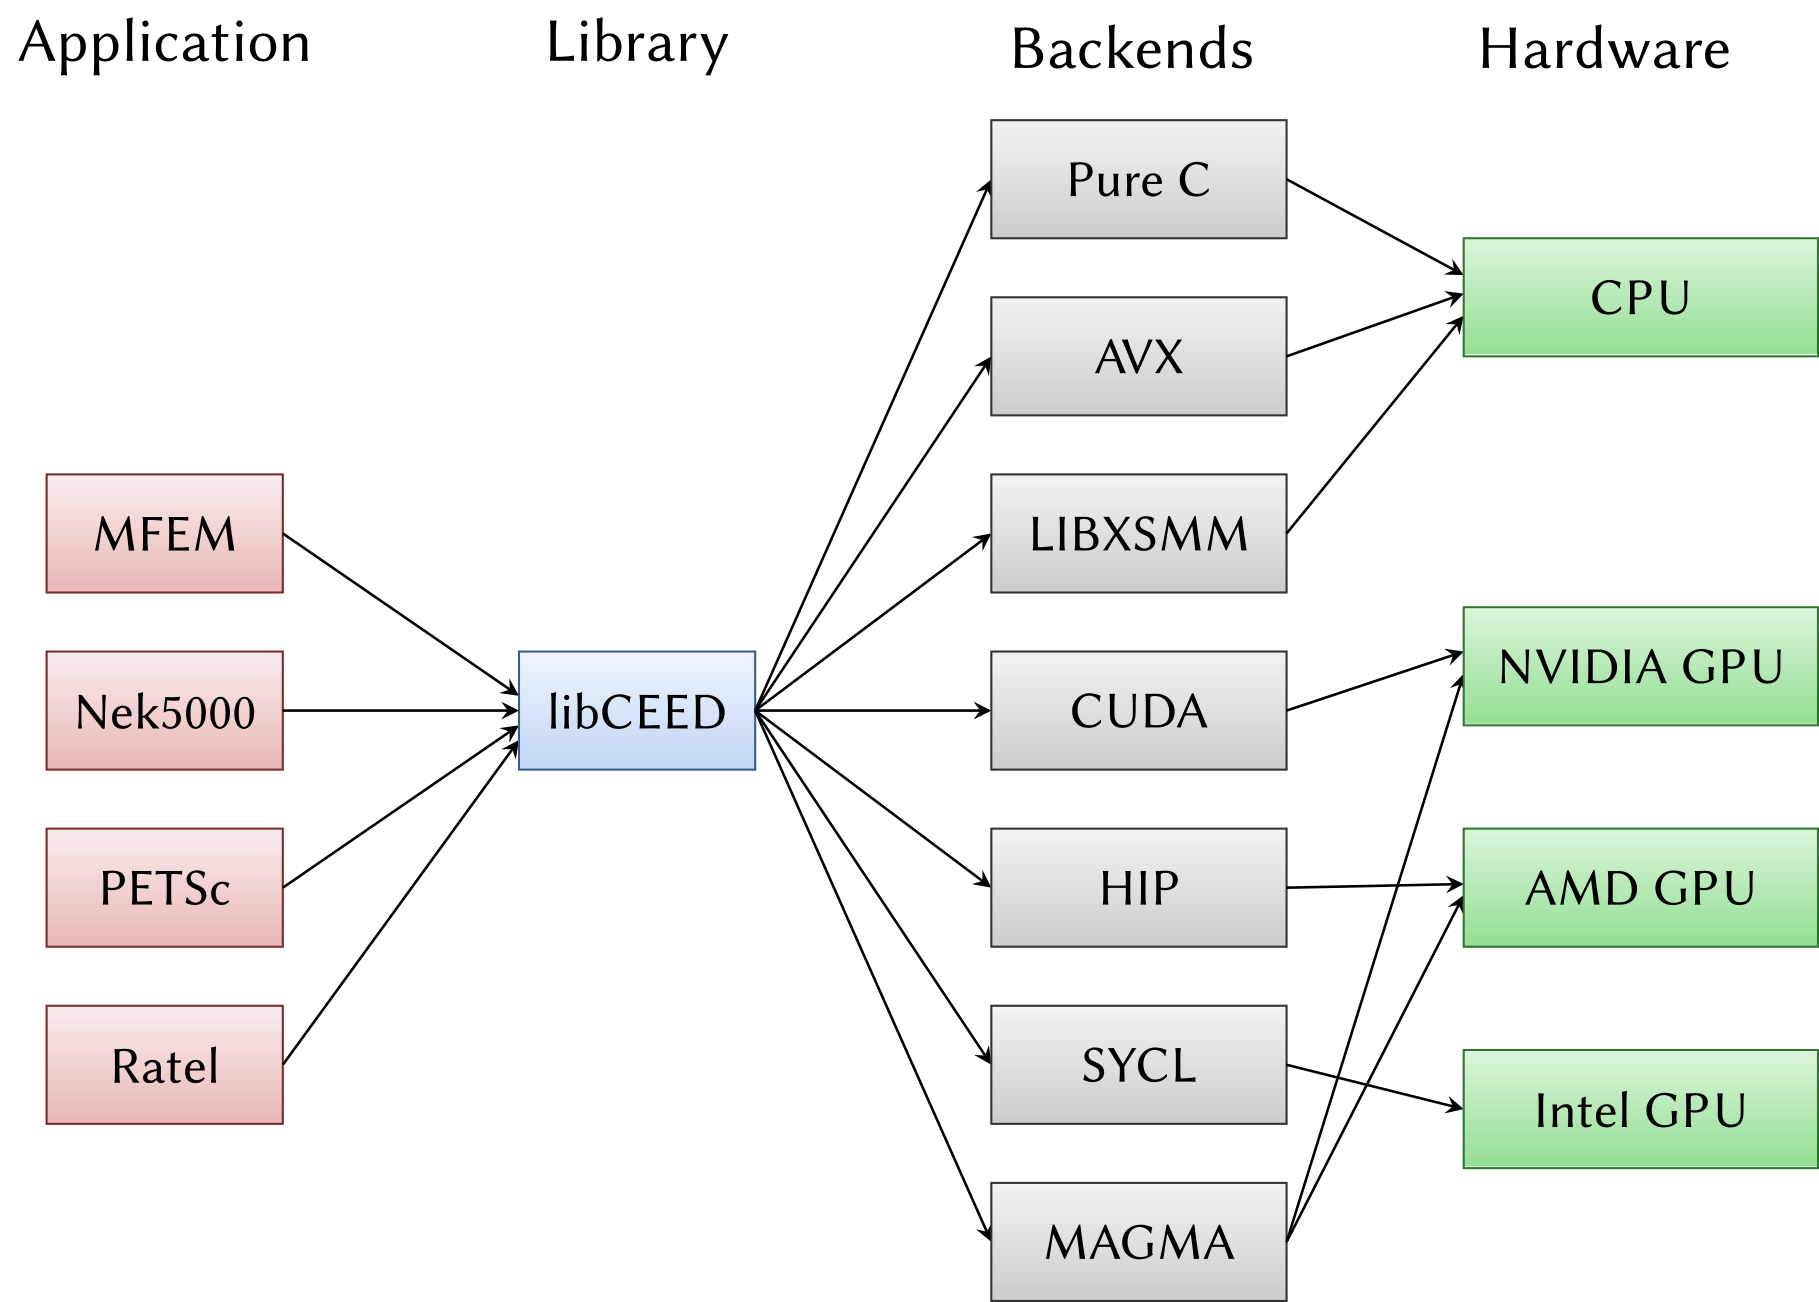
\includegraphics[height=5.5cm]{libCEEDBackends.png}

~\\

Performance portability with libCEED's matrix-free operators\\

\end{center}
\end{frame}

%------------------------------------------------

\begin{frame}
\begin{center}
\frametitle{Mini-Apps}

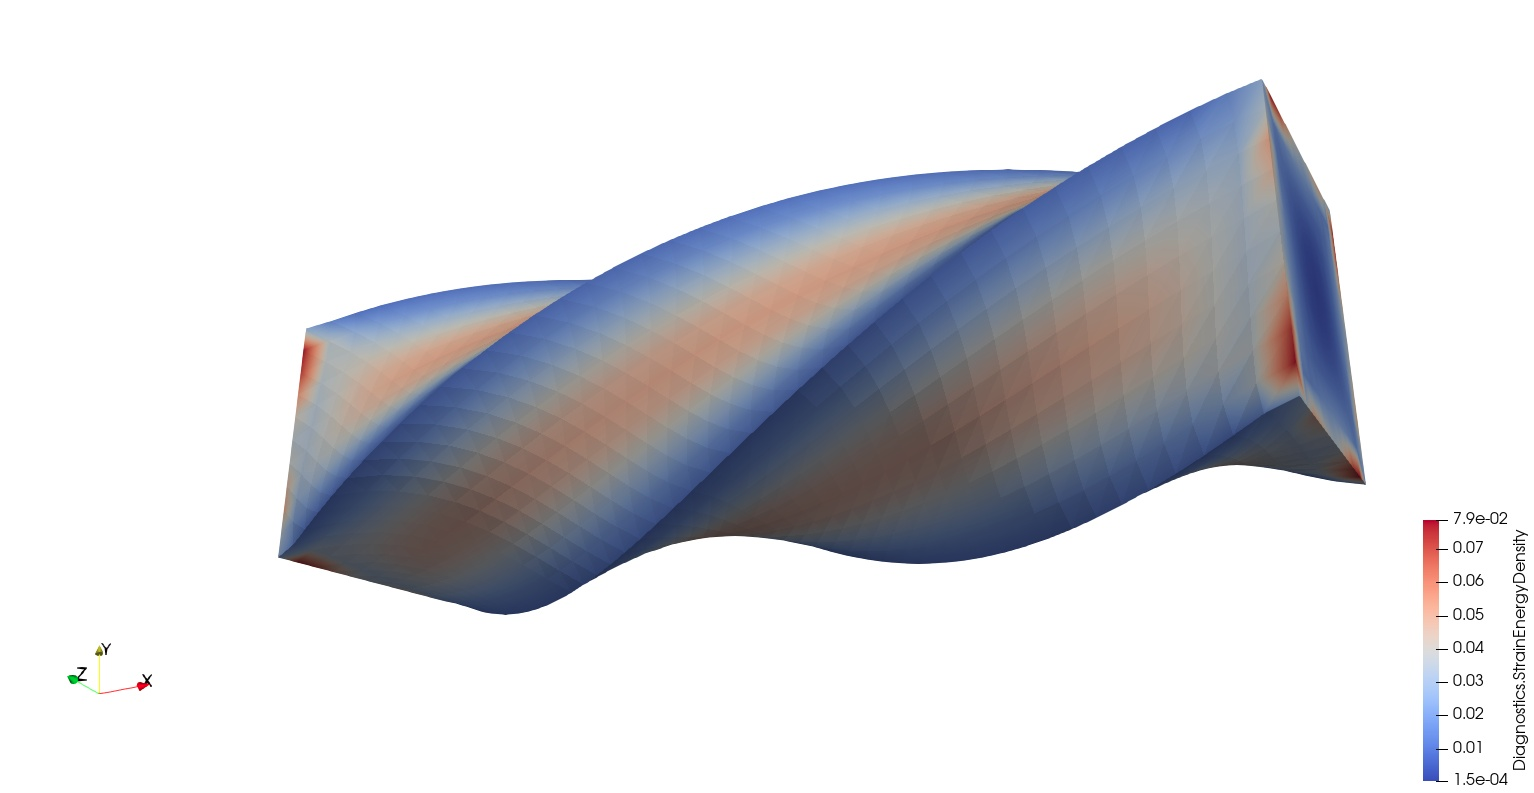
\includegraphics[height=3.2cm]{SolidTwistExample.png}
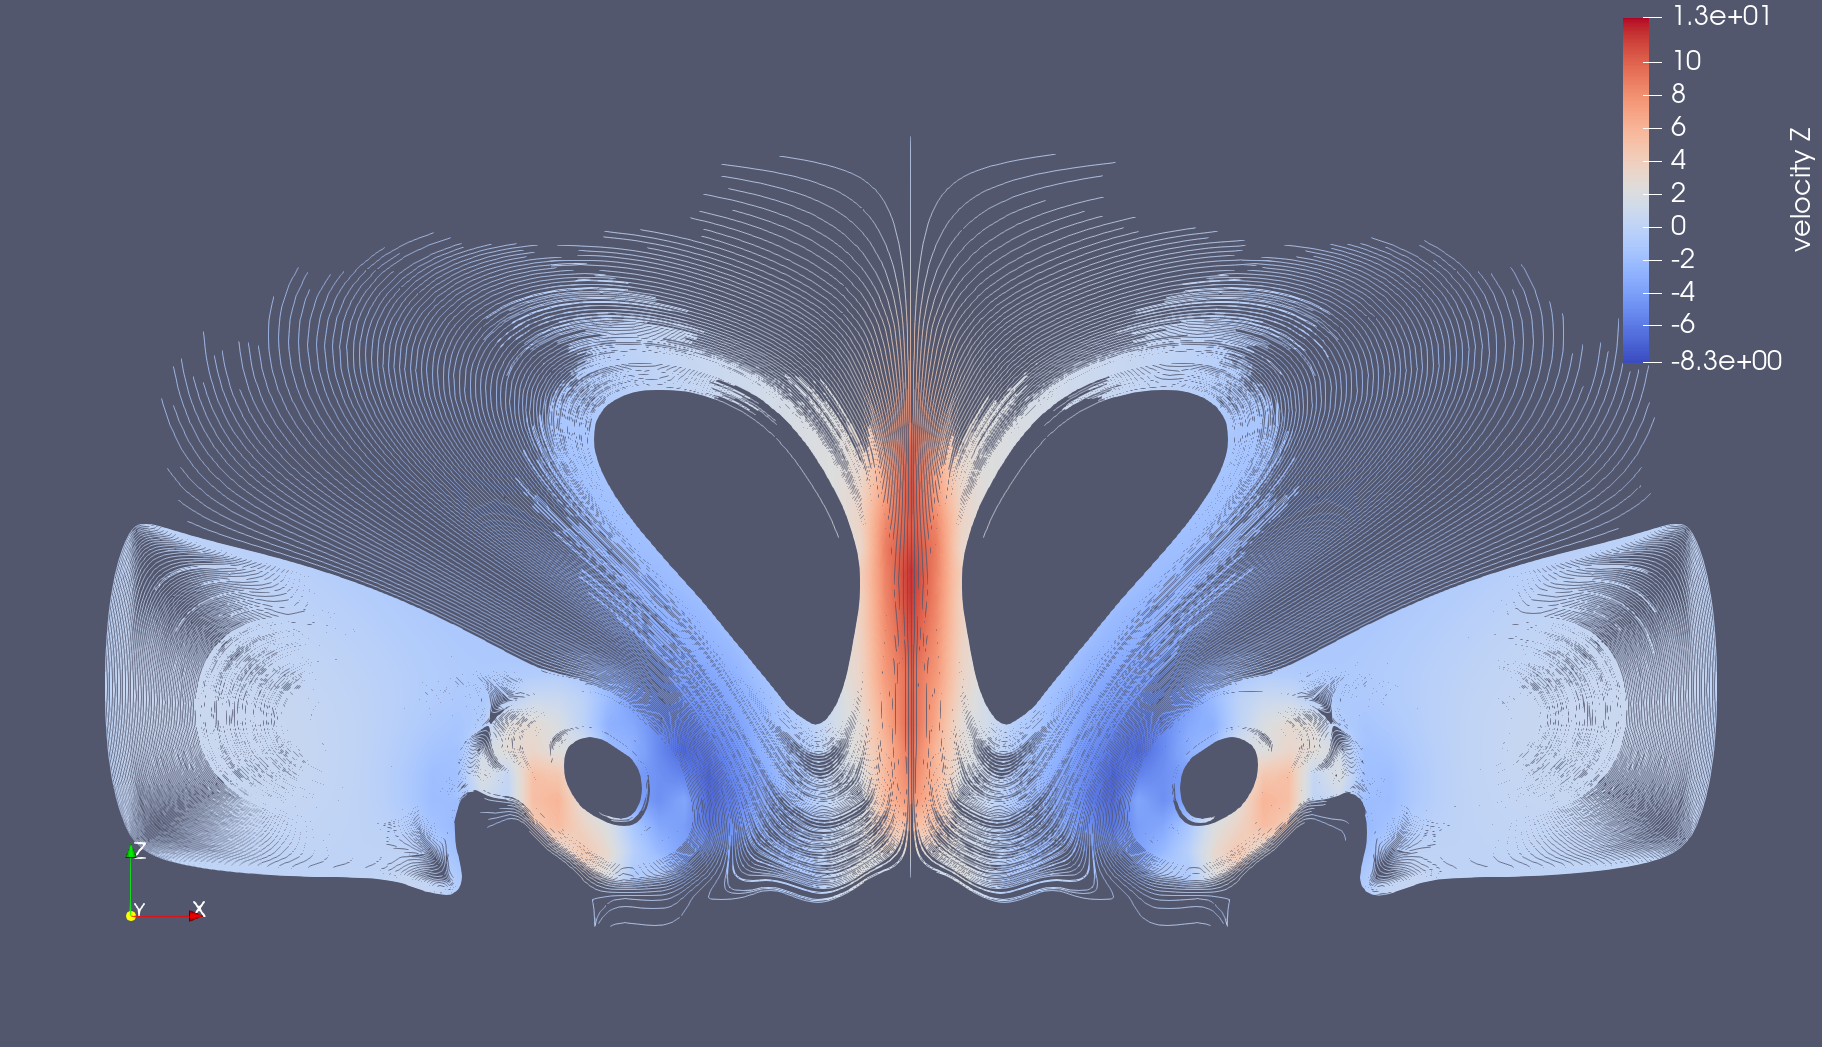
\includegraphics[height=3.2cm]{Vortices.png}

{\small libCEED solid mechanics (left) and fluid dynamics (right) mini-apps}

~\\

\begin{itemize}

\item libCEED supports FEM-like simulations on modern hardware

~\\

\item Mini-apps have been expanded into independent libraries

\end{itemize}

\end{center}
\end{frame}

%------------------------------------------------

\begin{frame}
\begin{center}
\frametitle{libCEED Projects}

Several projects built using libCEED\\

~\\

\begin{itemize}

\item Ratel - solid mechanics FEM and iMPM (PSAAP)\\

~\\

\item HONEE - fluid dynamics FEM \& differential filtering (PHASTA)\\

~\\

\item MFEM - various applications, libCEED integrators (LLNL)\\

~\\

\item Palace - quantum circuit design, MFEM + libCEED (Amazon)\\

~\\

\item RDycore - FV river dynamical core, PETSc + libCEED (SciDAC)\\

\end{itemize}

\end{center}
\end{frame}

%------------------------------------------------

\begin{frame}
\begin{center}
\frametitle{Design Implications}

Using matrix-free operators drives design decisions\\

~\\

\begin{itemize}

\item Direct solvers are out (assembled matrices, $\mathcal{O} \left( p^6 \right)$)\\

~\\

\item Iterative solvers are in (Krylov methods, etc)\\

~\\

\item High(er) order = high accuracy \& bad condition numbers\\

~\\

\item Preconditioning is needed for fast convergence\\

\end{itemize}

\end{center}
\end{frame}

%-------------------------------------------------------------------------------
\section{Ratel}
%-------------------------------------------------------------------------------

\begin{frame}
\frametitle{Ratel Team}

\begin{center}
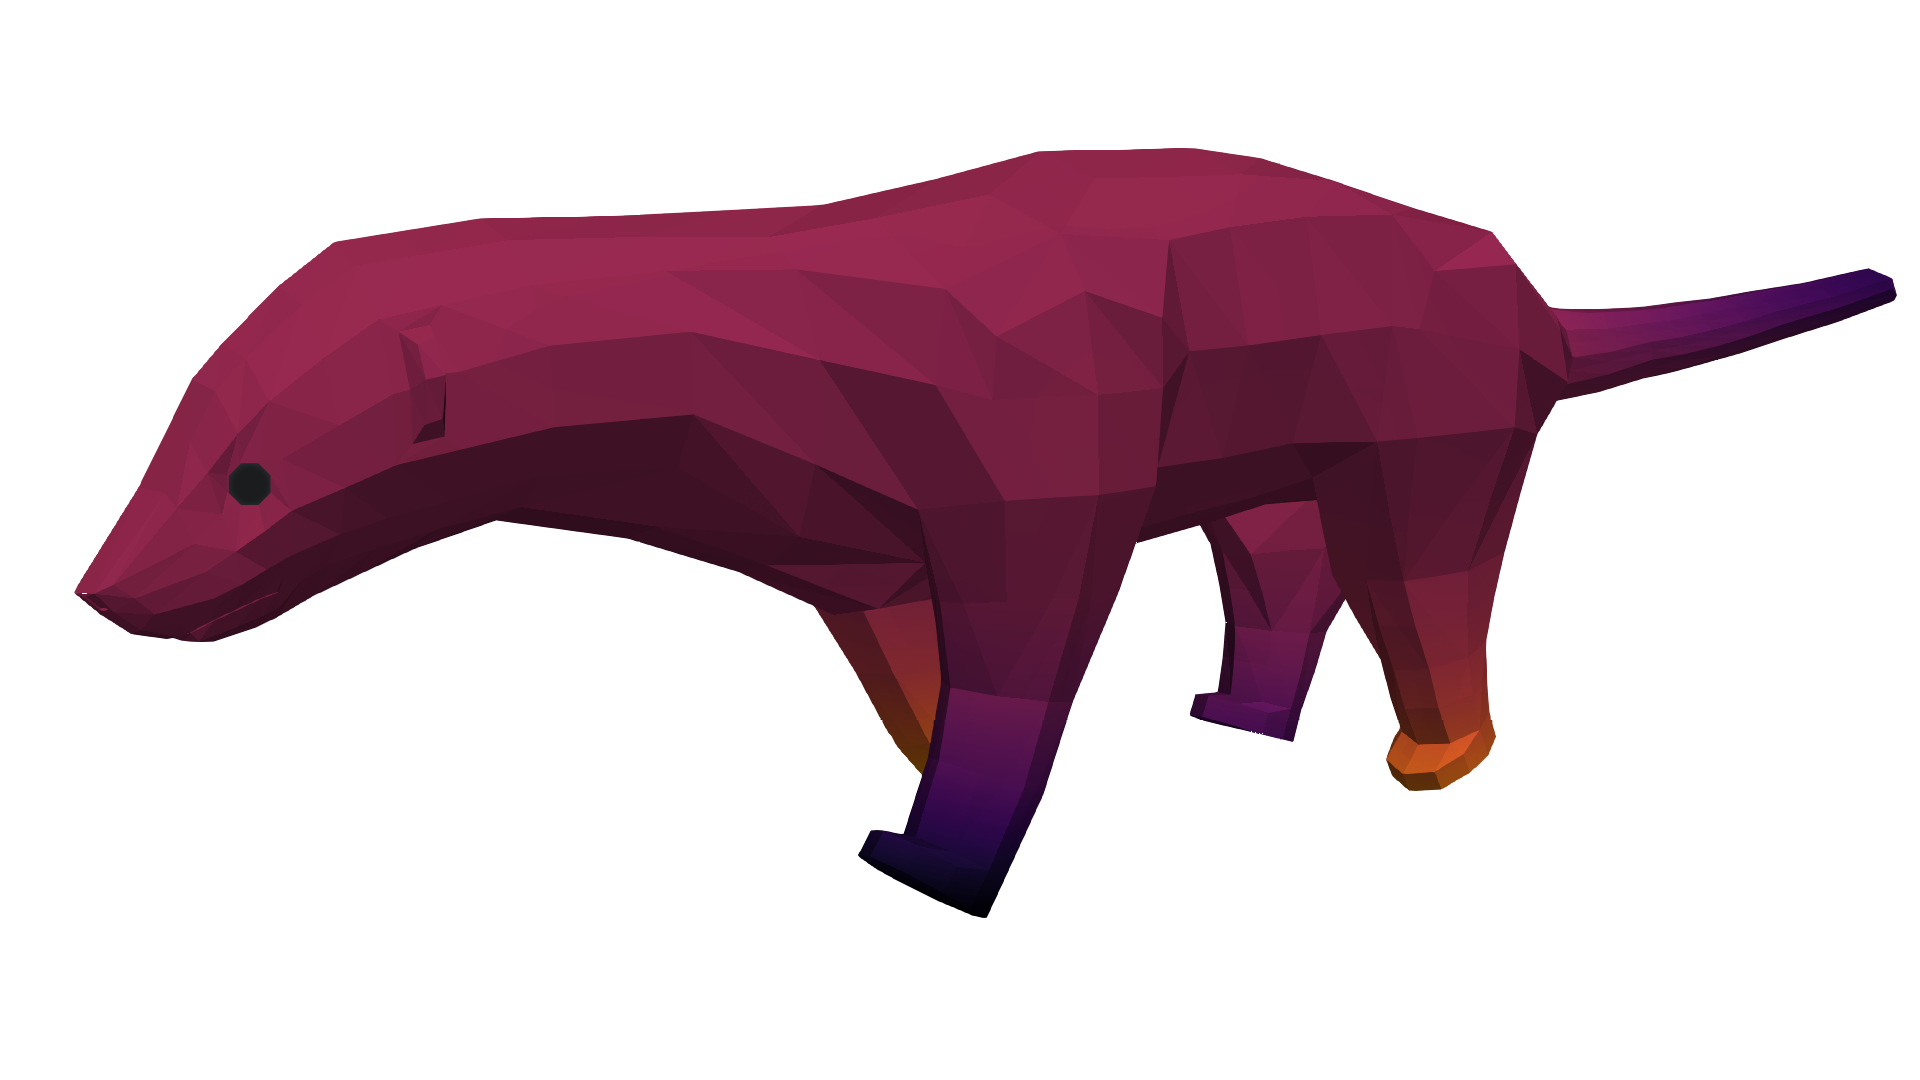
\includegraphics[height=2.75cm]{Ratellogo.png}
\end{center}

{\flushleft

Ratel Repo: \href{https://gitlab.com/micromorph/ratel}{https://gitlab.com/micromorph/ratel}\\

~\\
Developers: Zach R. Atkins, Jed Brown, Fabio Di Gioacchino,\\
\hspace{19mm} Leila Ghaffari, Zach Irwin, Rezgar Shakeri,\\
\hspace{19mm} Ren Stengel, Jeremy L Thompson\\

~\\

PSAAP Micromorph Center \& iMPM

}

\end{frame}

%------------------------------------------------

\begin{frame}
\begin{center}
\frametitle{Basic Design}

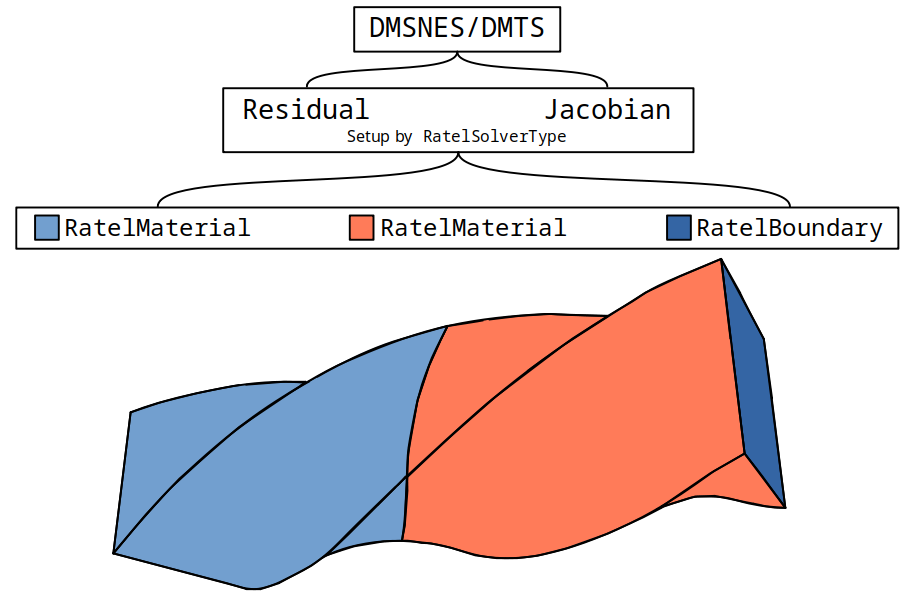
\includegraphics[height=5.5cm]{RatelAPI.png}

~\\

Each material region sets up part of the non-linear and linear equations\\

\end{center}
\end{frame}

%------------------------------------------------

\begin{frame}
\begin{center}
\frametitle{Material Models}

Multiple models are supported in Ratel\\

~\\

\begin{itemize}

\item Elasticity - Linear, Neo-Hookean, Mooney Rivlin, Ogden, Hencky\\

\item Mixed Elasticity - Linear, Neo-Hookean, Odgen\\

\item Plasticity - Hencky, various types\\

\item Anisostropy - Neo-Hookean\\

\item Brittle Fracture - Linear damage, Neo Hookean damage\\

\item Poromechanics - Linear, Neo-Hookean\\

\item Viscoelasticity - Hencky\\

\item iMPM - Neo-Hookean, Neo-Hookean damage\\

\end{itemize}

~\\

Current and initial configuration for many models\\


(Rezgar Shakeri, Fabio Di Gioacchino, Zach Irwin, PSAAP postdocs)

\end{center}
\end{frame}

%------------------------------------------------

\begin{frame}
\begin{center}
\frametitle{Boundary Conditions}

Multiple boundary conditions are supported in Ratel\\

~\\

\begin{itemize}

\item Clamp (Dirichlet)\\

\item Slip (partial Dirichlet)\\

\item Traction (Neumann)\\

\item Pressure\\

\item Rigid contact - Nitsche or penalty, with Coulomb or Threlfall friction\\

\end{itemize}

~\\

All BCs are time dependent\\


(Zach R. Atkins, PhD student and Rezgar Shakeri, PSAAP postdoc)

\end{center}
\end{frame}

%------------------------------------------------

\begin{frame}
\begin{center}
\frametitle{Preconditioning Support}

Iterative solvers need preconditioning\\

~\\

\begin{itemize}

\item $A x = b$, slow for high-order (ill-conditioned)\\

~\\

\item libCEED supports various preconditioner ingredients\\

~\\

\item Most PETSc preconditioners fully supported\\

~\\

\item Multigrid prolong/restrict also supported in libCEED\\

\end{itemize}

\end{center}
\end{frame}

%------------------------------------------------

\begin{frame}
\begin{center}
\frametitle{p-multigrid}

\begin{tikzpicture}
\node[shape=circle,draw=black] (A) at (0,0) {$p_2$};
\node[shape=circle] (Al) at (-1.2,0) {Smooth};
\node[shape=circle,draw=black] (B) at (2,-2) {$p_1$};
\node[shape=circle] (Bl) at (0.8,-2) {Smooth};
\node[shape=circle,draw=black] (C) at (4,-4) {$p_0$};
\node[shape=circle] (Cl) at (4,-5) {Coarse Solve};
\node[shape=circle,draw=black] (D) at (6,-2) {$p_1$};
\node[shape=circle] (Dl) at (7.2,-2) {Smooth};
\node[shape=circle,draw=black] (E) at (8,0) {$p_2$};
\node[shape=circle] (El) at (9.2,0) {Smooth};
\path[->] (A) edge node[left=10, pos=.6] {Restriction} (B);
\path[->] (B) edge node[left=10, pos=.6] {Restriction} (C);
\path[->] (C) edge node[right=10, pos=.4] {Interpolation} (D);
\path[->] (D) edge node[right=10, pos=.4] {Interpolation} (E);
\end{tikzpicture}

\vspace{-0.9cm}

Ratel uses matrix-free p-multigrid, AMG coarse solve\\

\end{center}
\end{frame}

%------------------------------------------------

\begin{frame}[fragile]
\begin{center}
\frametitle{Example - Linear Damage}

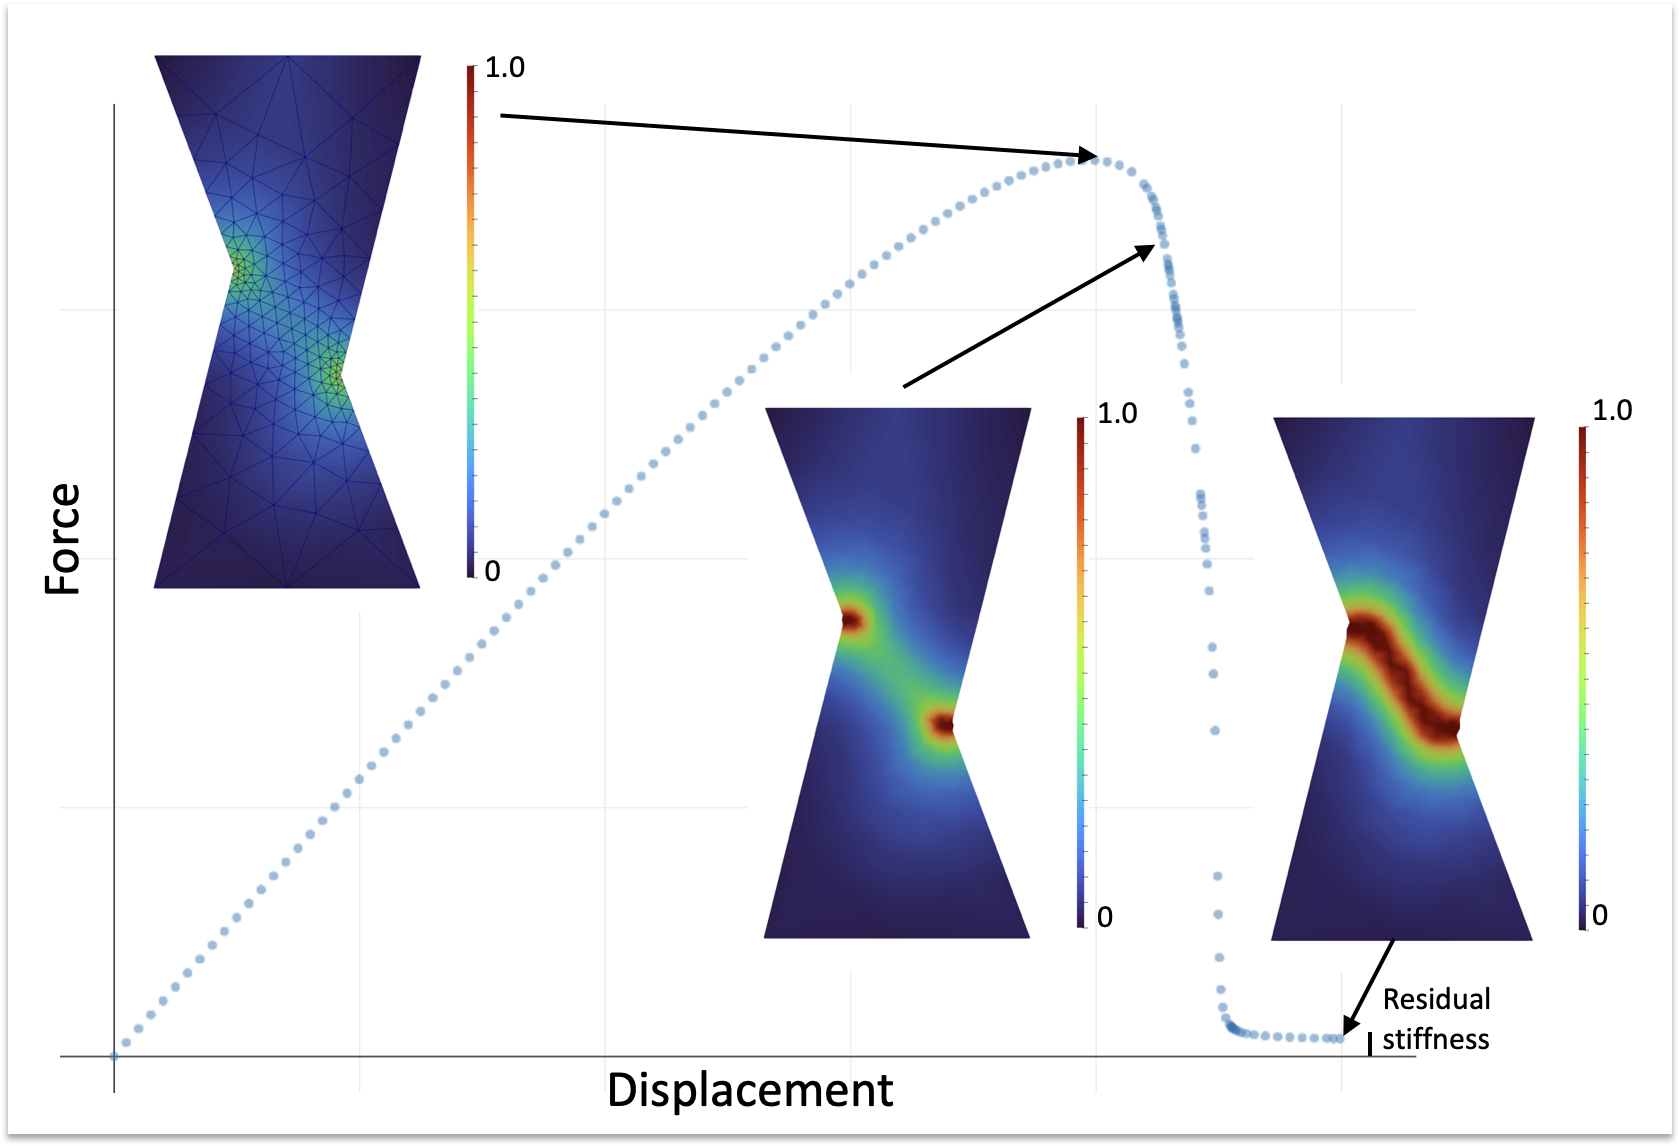
\includegraphics[height=4.5cm]{compressive-shear-damage-FEM.png}

{\tiny
\begin{lstlisting}
$ bin/ratel-quasistatic -options_file examples/ymls/ex02-quasistatic-elasticity-linear-damage-compressiveshear-AT2-face-forces.yml
\end{lstlisting}
}

Quasistatic simulation of compressive shear for generic brittle material\\


(Fabio Di Gioacchino, PSAAP postdoc)

\end{center}
\end{frame}

%------------------------------------------------

\begin{frame}[fragile]
\begin{center}
\frametitle{Example - Hencky Viscoelasticity Damage}

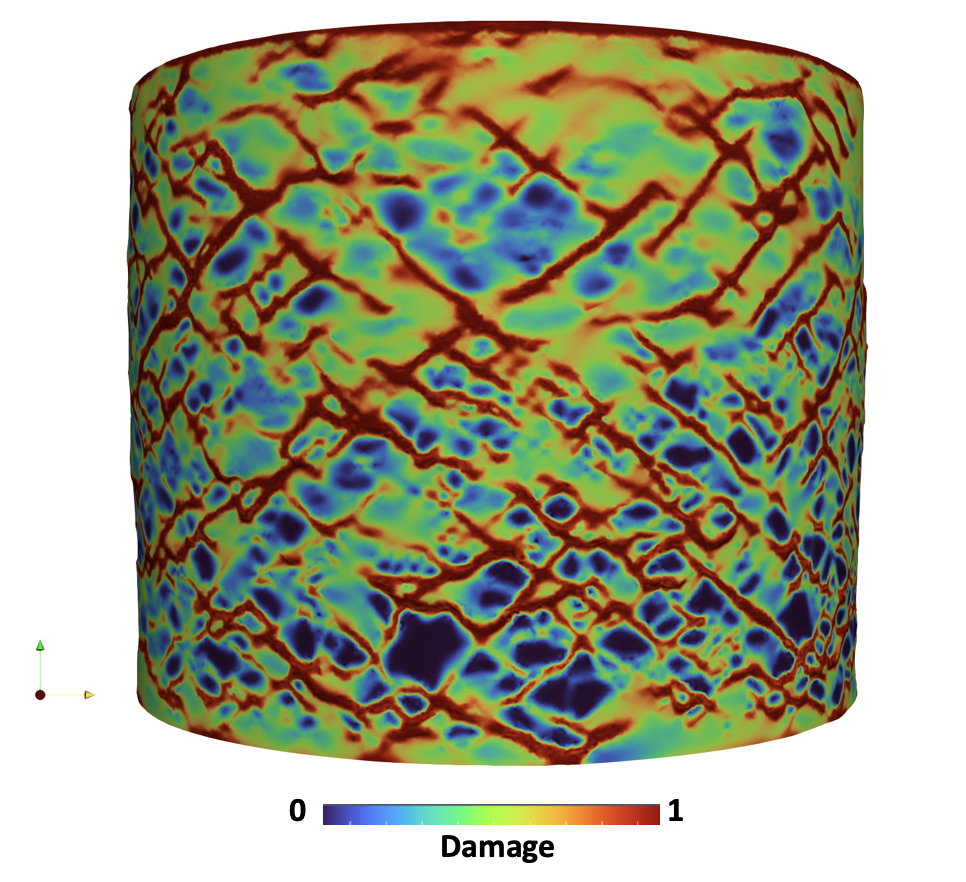
\includegraphics[height=5cm]{HenckyViscoDamage.png}

Quasistatic simulation of IDOX grains in IDOX/Estane matrix\\
with damage due to unconfined compression\\

~\\

(Fabio Di Gioacchino, PSAAP postdoc)

\end{center}
\end{frame}

%------------------------------------------------

\begin{frame}[fragile]
\begin{center}
\frametitle{Example - Dynamic Pendulum}

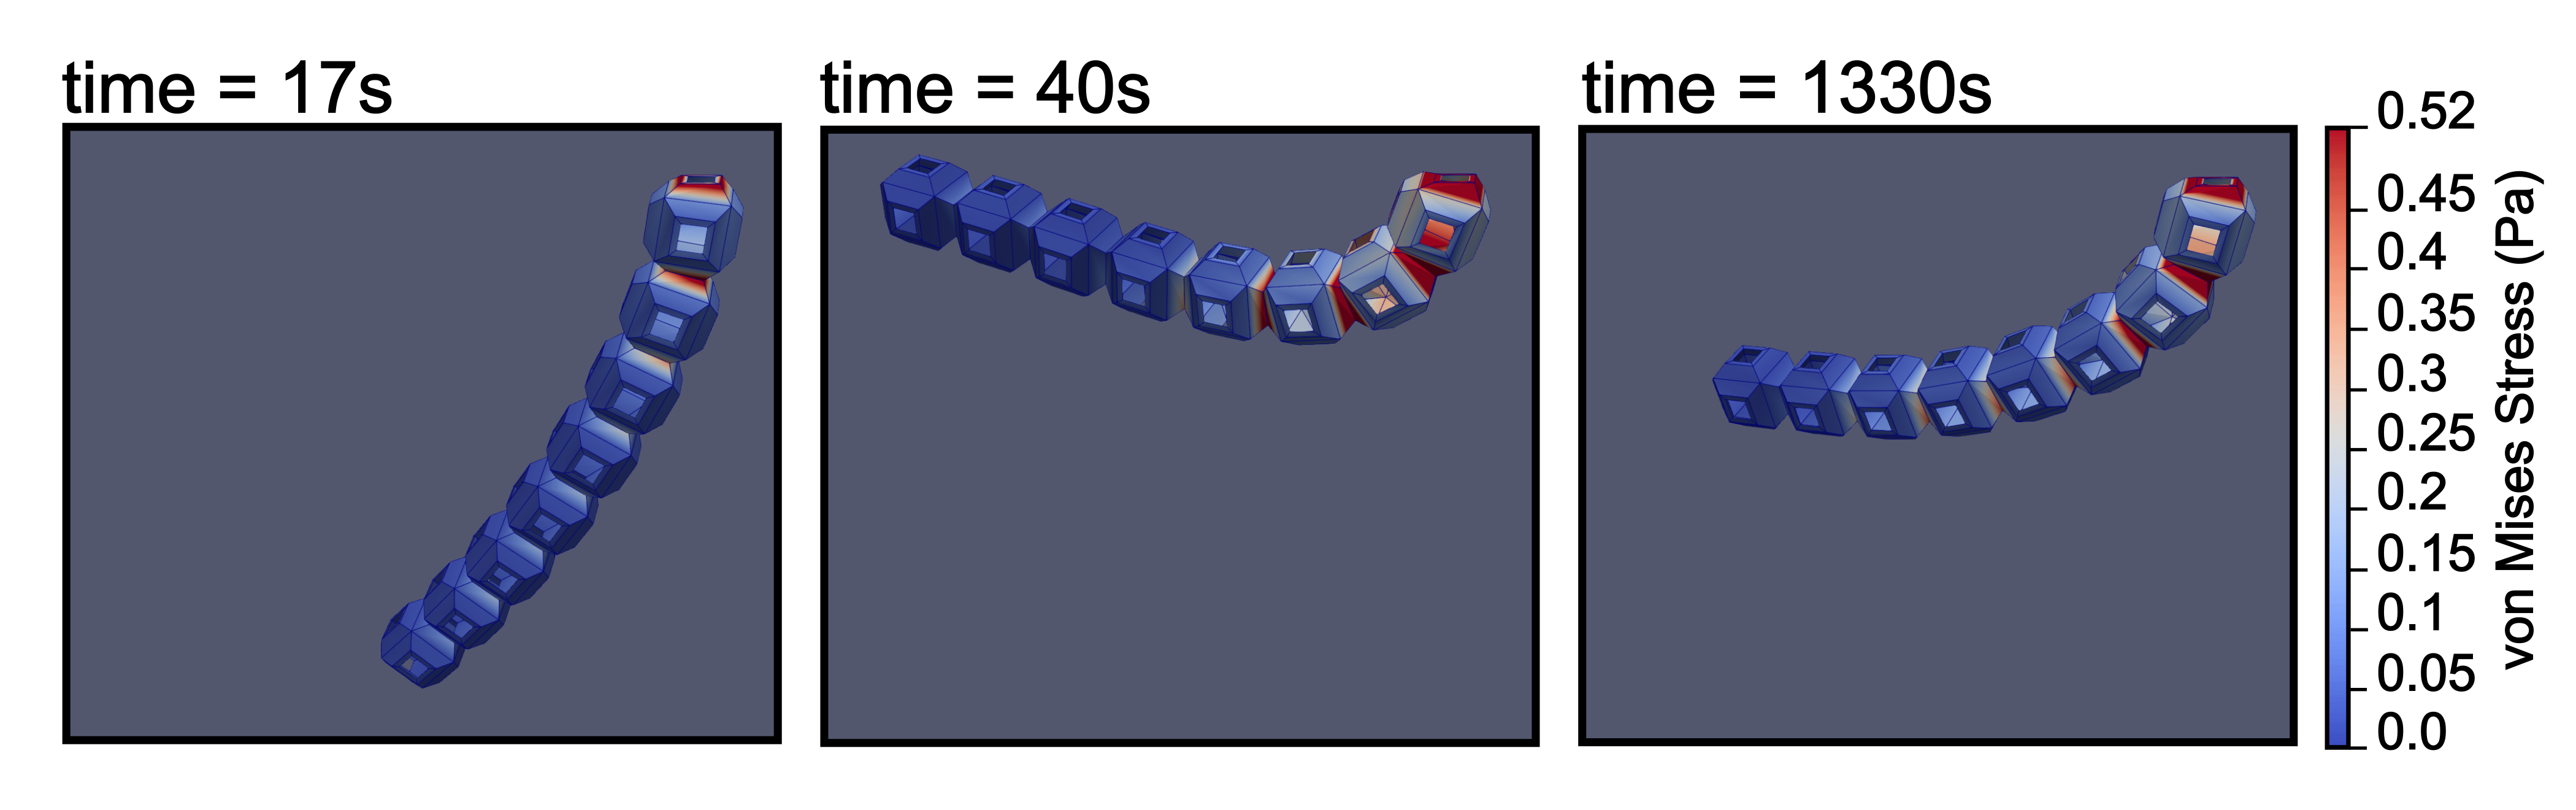
\includegraphics[height=3.8cm]{dynamic-pendulum.png}

{\tiny
\begin{lstlisting}
$ bin/ratel-dynamic -options_file examples/ymls/ex03-dynamic-elasticity-schwarz-pendulum-enzyme.yml
\end{lstlisting}
}

Dynamic simulation of Neo-Hookean Schwarz-P 'pendulum' with Enzyme

(Layla Ghaffari, recent PhD graduate)

\end{center}
\end{frame}

%------------------------------------------------

\begin{frame}
\begin{center}
\frametitle{CEED Benchmark Problems}

Performance on CEED BPs

~\\

\begin{itemize}

\item BP1 - Scalar projection problem\\

~\\

\item BP2 - 3 component projection problem\\

~\\

\item BP3 - Scalar Poisson problem\\

~\\

\item BP4 - 3 component Poisson problem\\

~\\

\item Ogden - representative production problem\\

\end{itemize}

~\\

Bulk of FLOPs are in basis evaluation for BPs

\end{center}
\end{frame}

%------------------------------------------------

\begin{frame}
\begin{center}
\frametitle{CEED Benchmark Problems}

Performance on CEED BPs

~\\

\begin{itemize}

\item $p = 2, 3, 4$ and $q = p + 1$\\

~\\

\item Units cube with $30^3$, $60^3$, $90^3$, $120^3$, and $150^3$ elements\\

~\\

\item Compare tensor, non-tensor, and at-points basis evaluation\\

~\\

\item MMS w/ partial sum of Weierstrass function, $a = 0.5$, $b = 1.5$, $N = 2$\\

\end{itemize}

~\\

Using 4x AMD Instinct\texttrademark MI300A Accelerated Processing Units (APUs)\\

~\\

See also Performance Portable Solid mechanics via Matrix-Free p-Multigrid\\

(Also, dissertation of Ren Stengel, recent PhD graduate)

\end{center}
\end{frame}

%------------------------------------------------

\begin{frame}
\begin{center}
\frametitle{BP1}

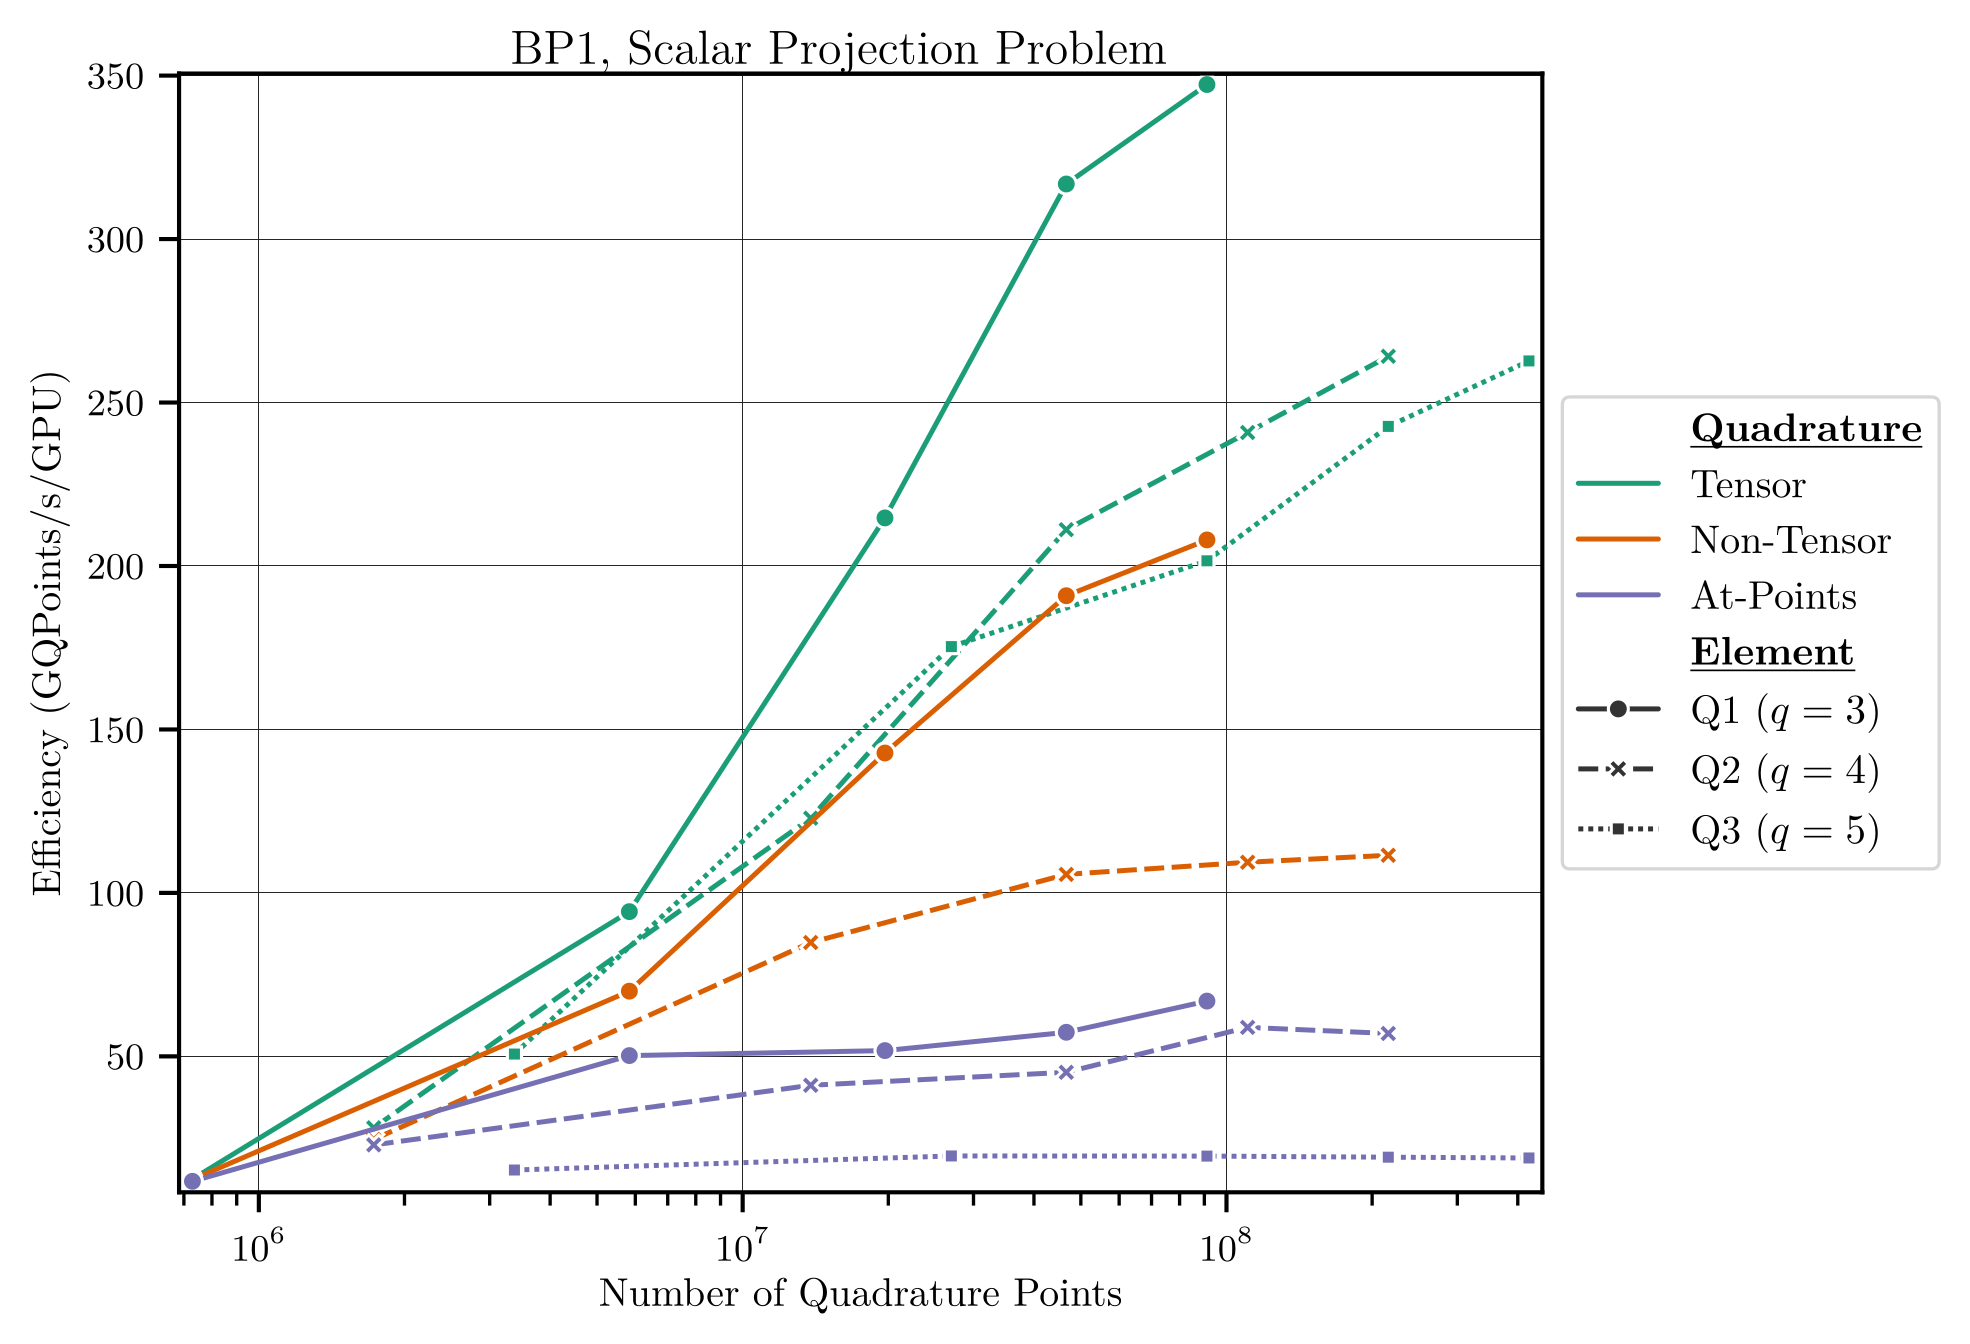
\includegraphics[height=6.5cm]{Ratel_BP1.png}\\

~\\

More FLOPs to do leads to lower efficiency

\end{center}
\end{frame}

%------------------------------------------------

\begin{frame}
\begin{center}
\frametitle{BP2}

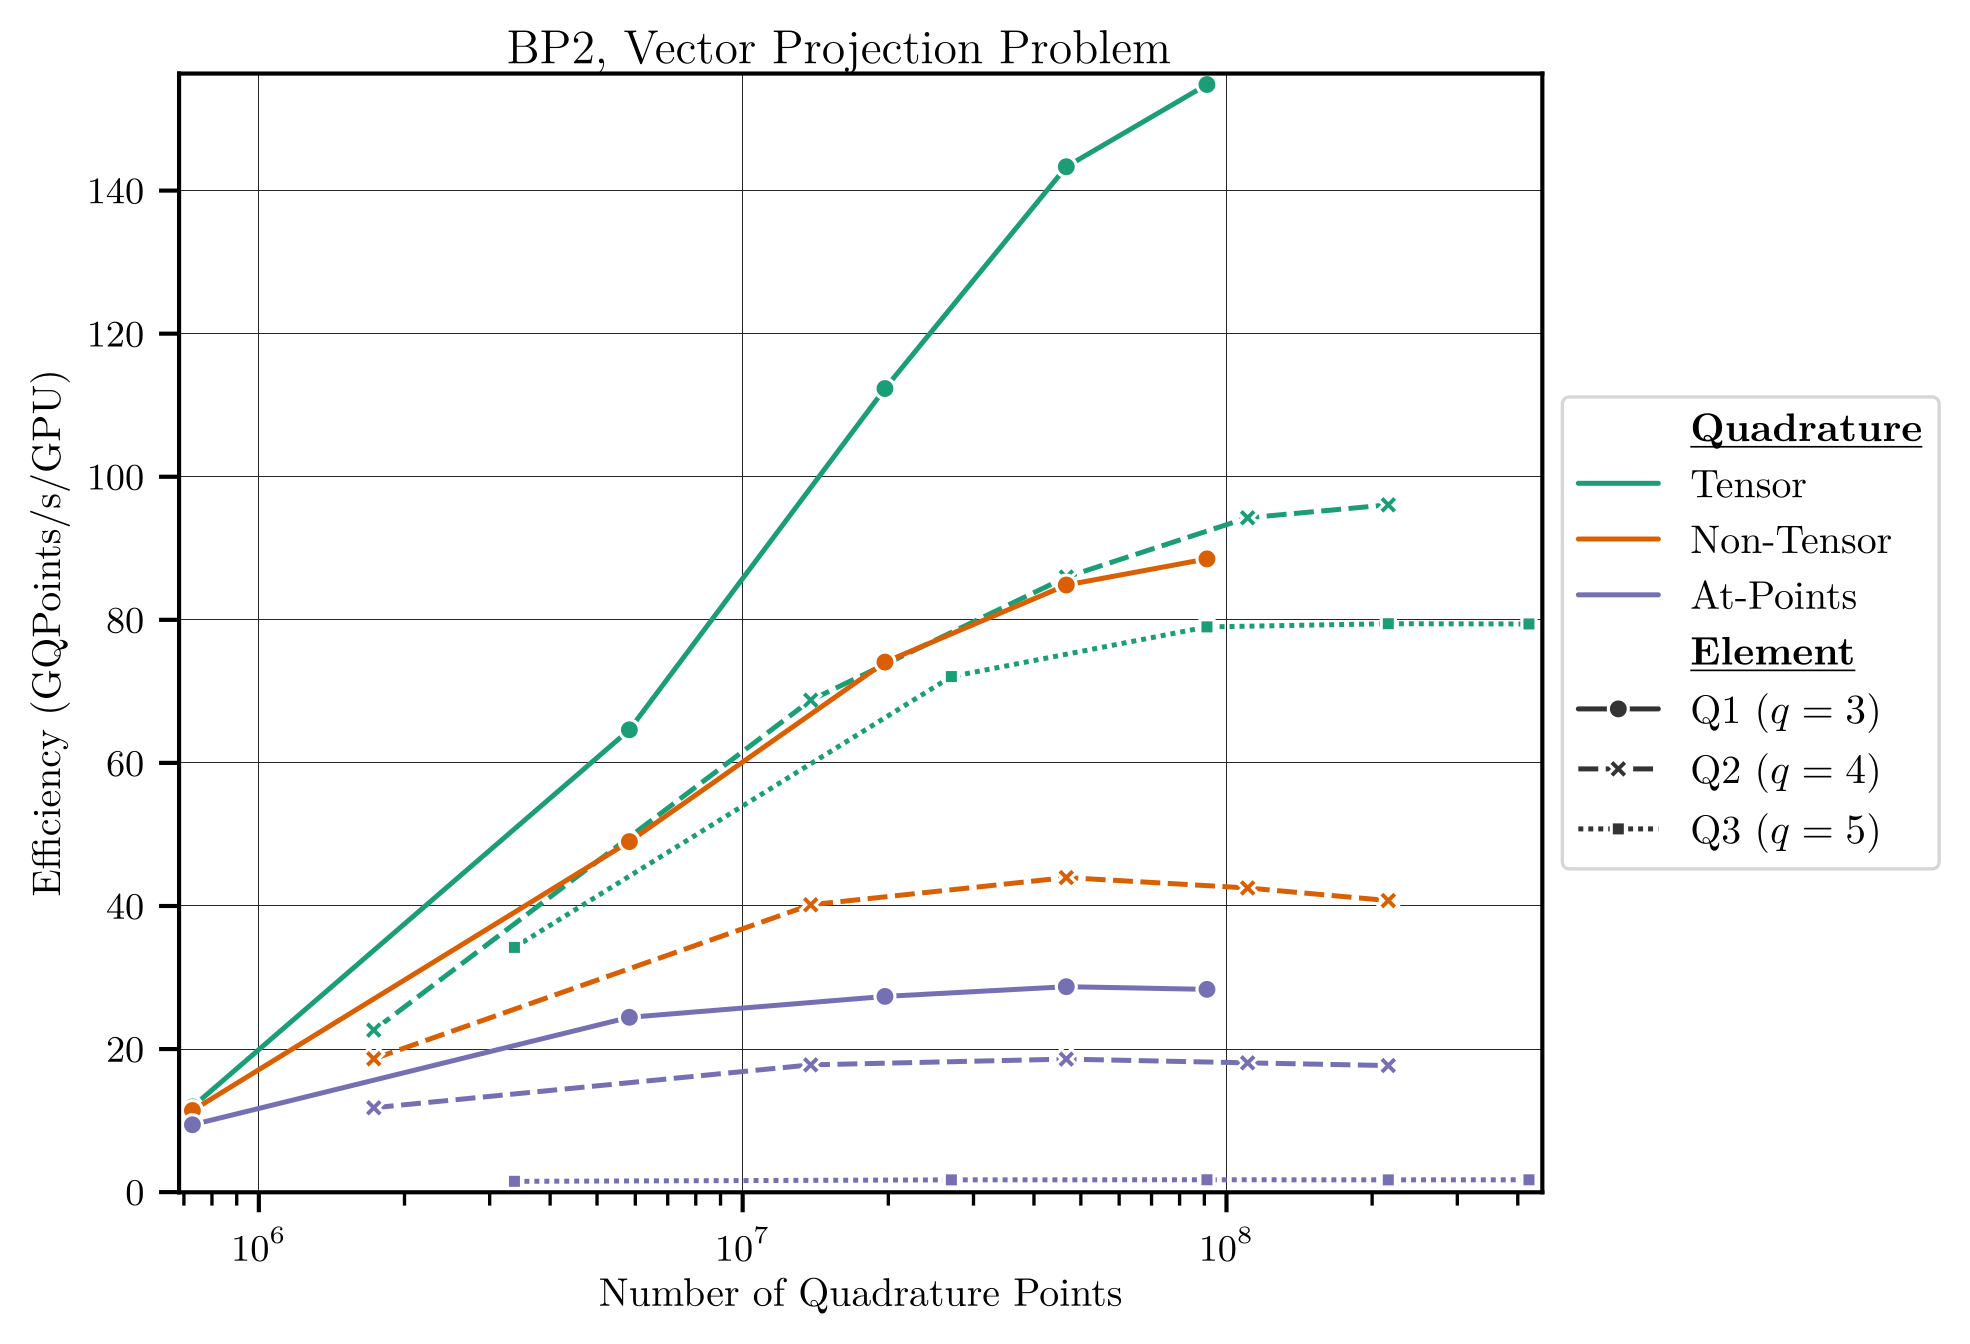
\includegraphics[height=6.5cm]{Ratel_BP2.png}\\

~\\

More components better represents production workloads

\end{center}
\end{frame}

%------------------------------------------------

\begin{frame}
\begin{center}
\frametitle{BP3}

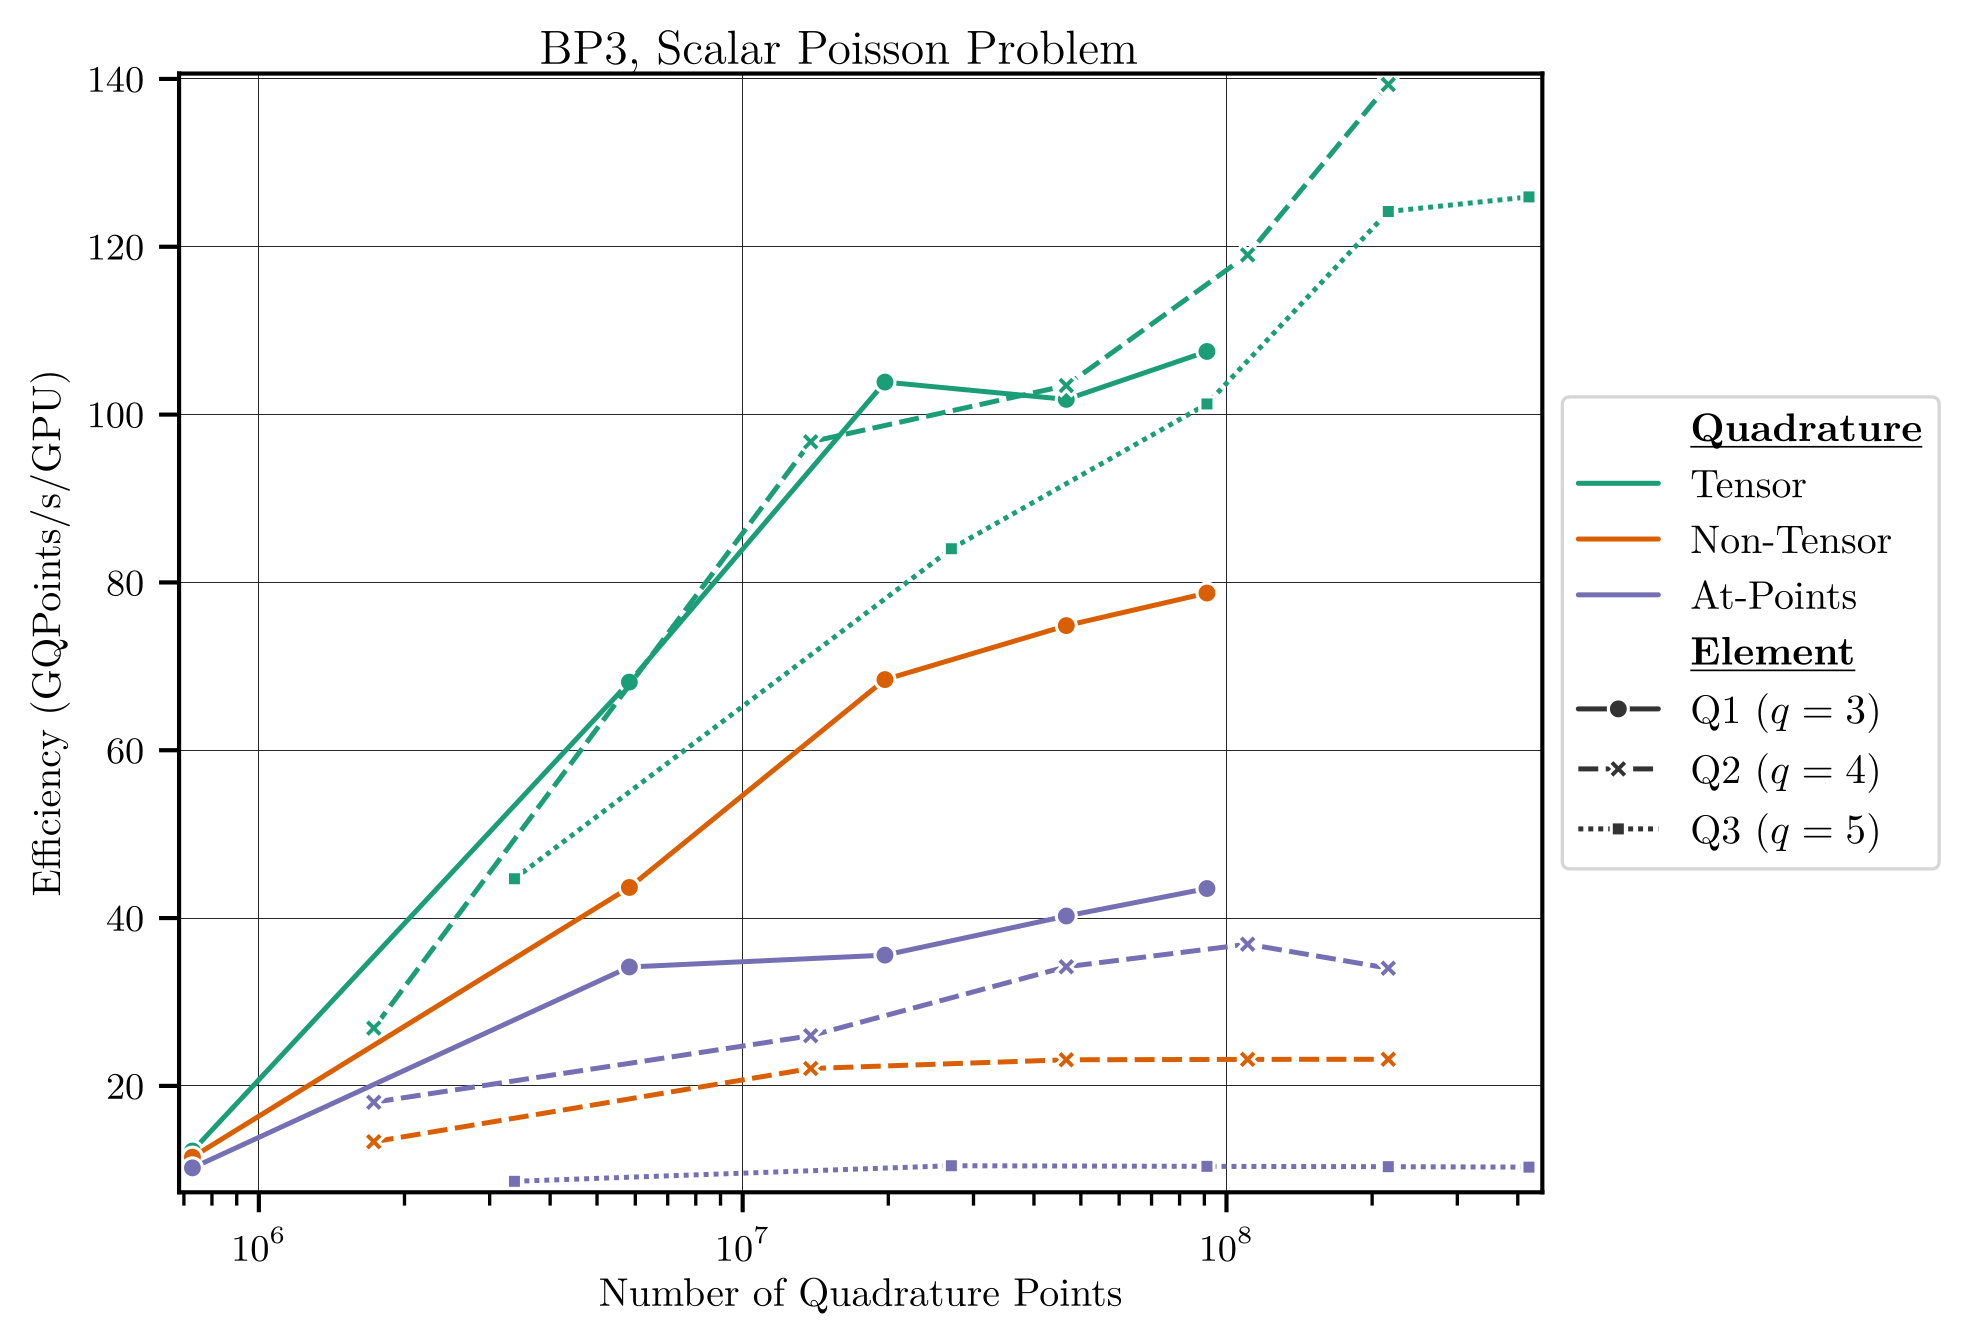
\includegraphics[height=6.5cm]{Ratel_BP3.png}\\

~\\

With derivatives, at-points closer to non-tensor

\end{center}
\end{frame}

%------------------------------------------------

\begin{frame}
\begin{center}
\frametitle{BP4}

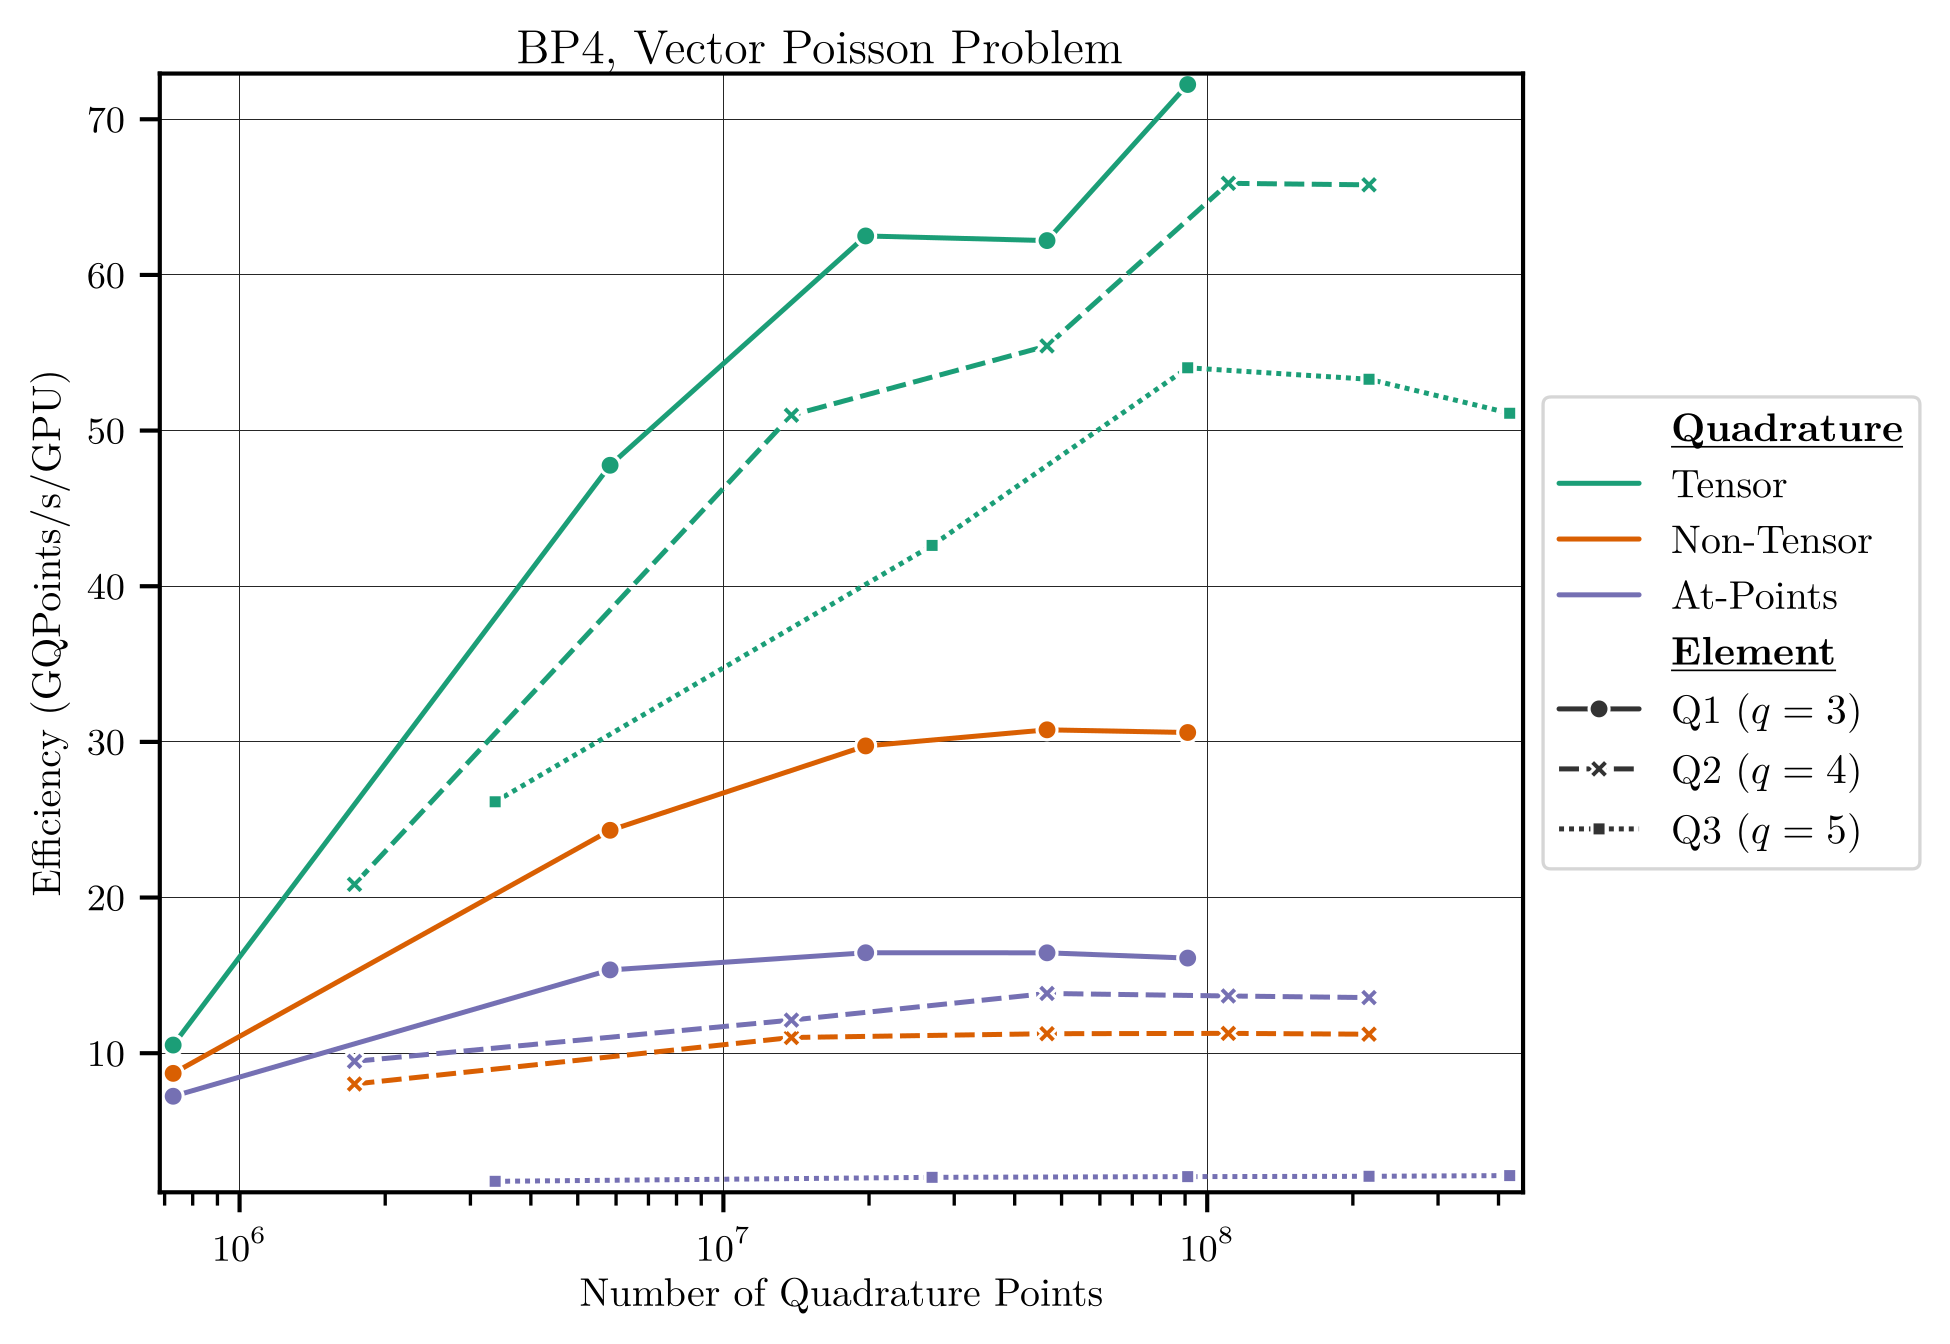
\includegraphics[height=6.5cm]{Ratel_BP4.png}\\

~\\

Closest CEED BP to production workload

\end{center}
\end{frame}

%------------------------------------------------

\begin{frame}
\begin{center}
\frametitle{Ogden}

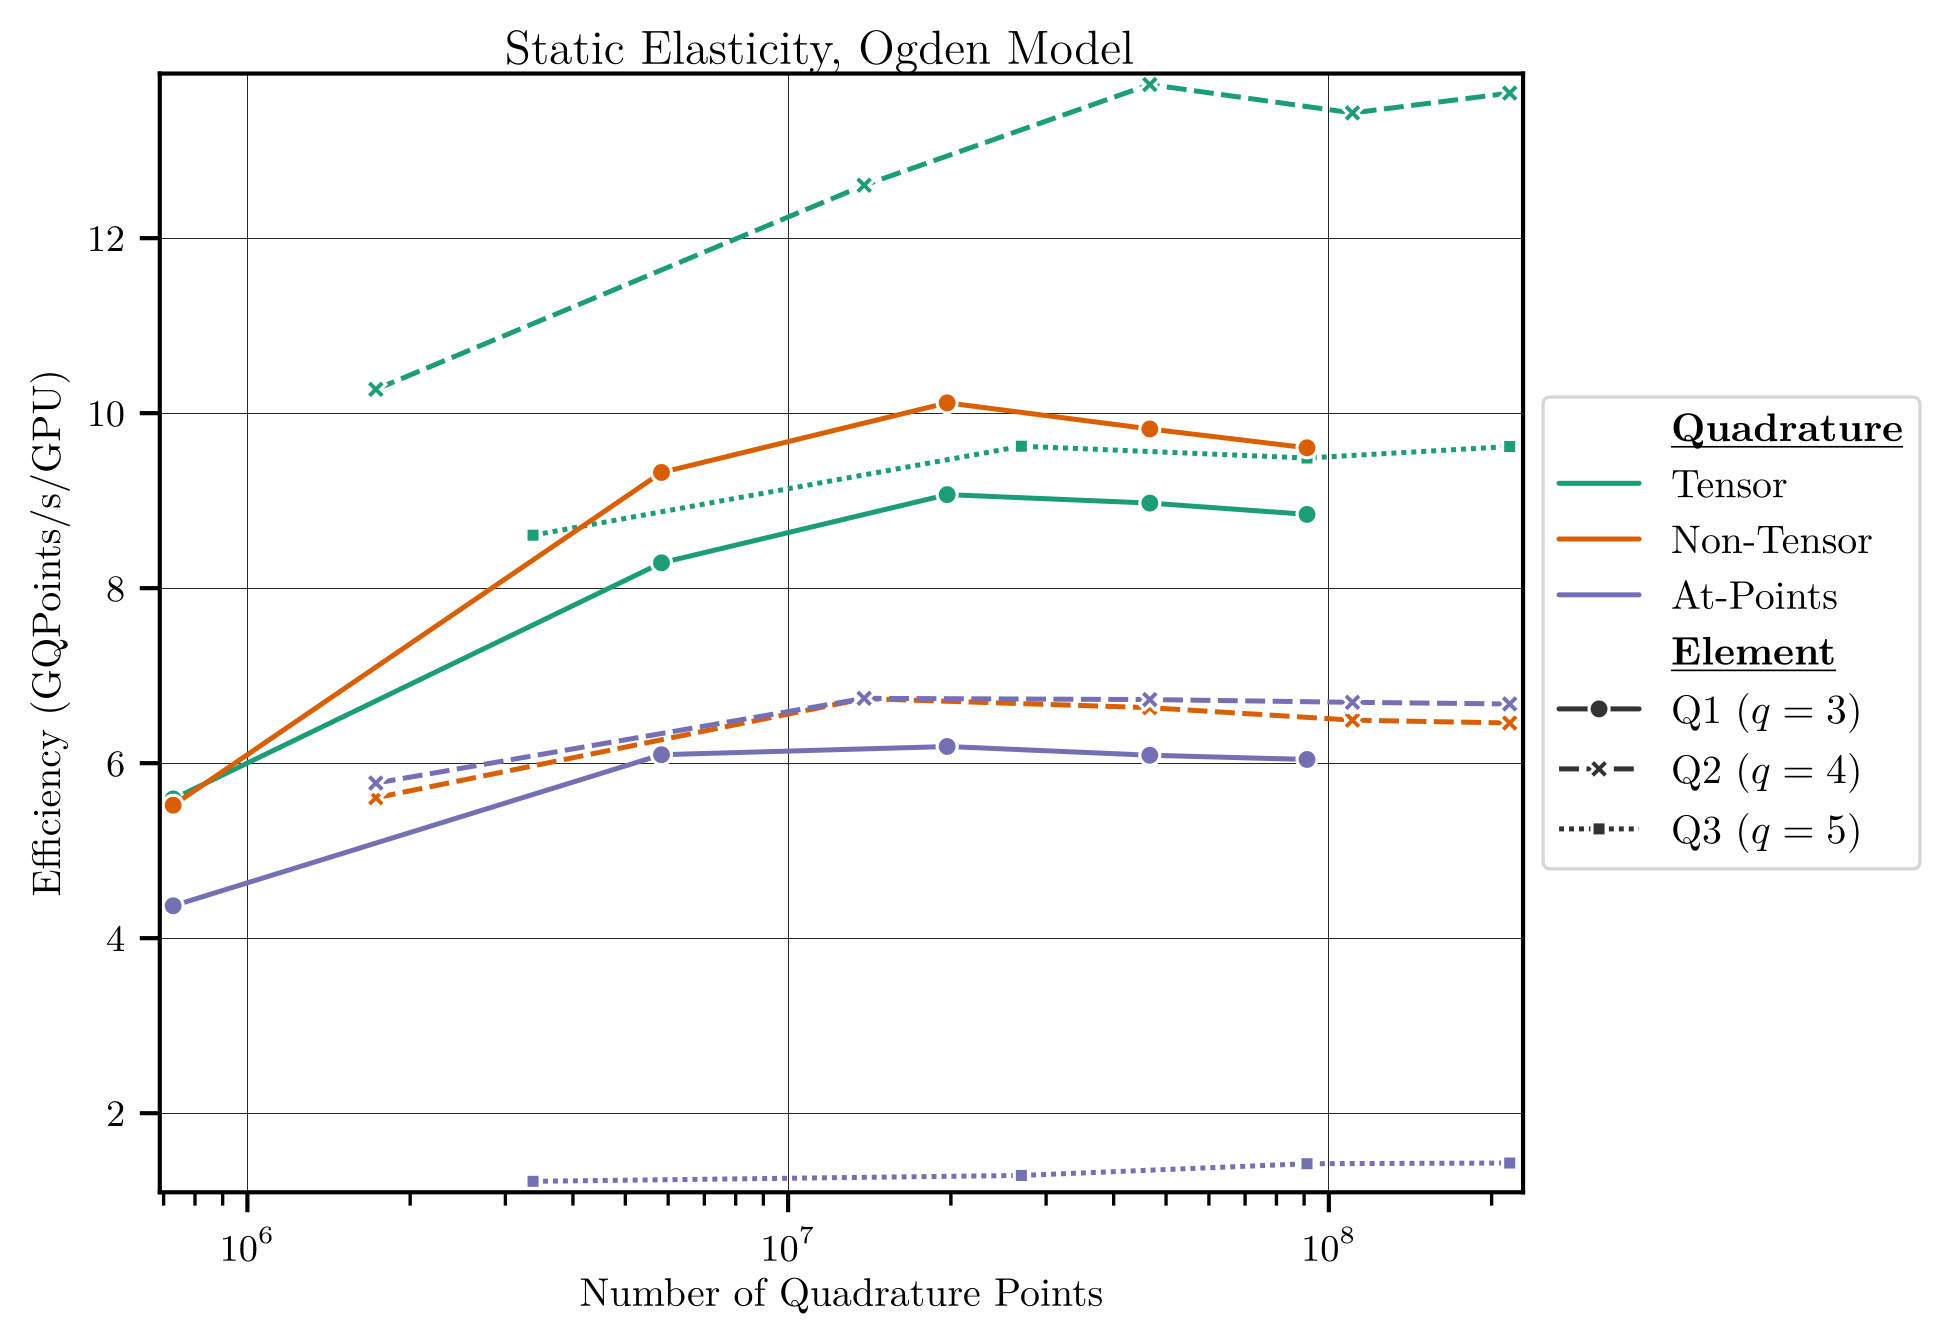
\includegraphics[height=6.5cm]{Ratel_Ogden.png}\\

~\\

Basis cost less important with heavier QFunctions

\end{center}
\end{frame}

%-------------------------------------------------------------------------------
\section{GPU and AD}
%-------------------------------------------------------------------------------

\begin{frame}[fragile]
\begin{center}
\frametitle{Two Families of Approaches}

Three libCEED backends with two approaches to operator application\\

~\\

\begin{itemize}

\item Separate kernels

\begin{itemize}

\item \lstinline{/gpu/*/ref} and \lstinline{/gpu/*/shared}\\

~\\

\item $\mathcal{E}$, {\color{blue(ncs)}$B$}, and {\color{applegreen}$D$} all separate kernels\\

~\\

\item Higher overall memory usage, multiple kernel launches\\

~\\

\end{itemize}

\item Fused kernel

\begin{itemize}

\item \lstinline{/gpu/*/gen}\\

~\\

\item Single kernel JiTed with data from $\mathcal{E}$, {\color{blue(ncs)}$B$}, and {\color{applegreen}$D$}\\

~\\

\item Lower overall memory usage, single kernel launch\\

\end{itemize}

\end{itemize}

\end{center}
\end{frame}

%------------------------------------------------

\begin{frame}[fragile]
\begin{center}
\frametitle{Ref Operator Application}

\lstinline{/gpu/*/ref} and \lstinline{/gpu/*/shared} use largely the same code\\

~\\

${\color{burgundy}A}_L = \mathcal{E}^T {\color{blue(ncs)}B}^T {\color{applegreen}D} {\color{blue(ncs)}B} \mathcal{E}$ use separate kernels\\

~\\

$\mathcal{E}$ source comes from the \lstinline{/gpu/*/ref}\\

~\\

\lstinline{/gpu/*/ref} uses basic kernels for {\color{blue(ncs)}$B$}\\

~\\

\lstinline{/gpu/*/shared} uses shared memory for {\color{blue(ncs)}$B$}\\

~\\

{\color{applegreen}$D$} source is given by the user\\

\end{center}
\end{frame}

%------------------------------------------------

\begin{frame}[fragile]
\begin{center}
\frametitle{Gen Operator Application}

\lstinline{/gpu/*/gen} generates a single kernel for the operator\\

~\\

${\color{burgundy}A}_L = \mathcal{E}^T {\color{blue(ncs)}B}^T {\color{applegreen}D} {\color{blue(ncs)}B} \mathcal{E}$ uses a single kernel\\

~\\

$\mathcal{E}$ source comes from the \lstinline{/gpu/*/ref}\\

~\\

{\color{blue(ncs)}$B$} source comes from \lstinline{/gpu/*/shared}\\

~\\

{\color{applegreen}$D$} source is given by the user\\

~\\

~\\

(Original gen backend by Yohann Dudouit)

\end{center}
\end{frame}

%------------------------------------------------

\begin{frame}[fragile]
\begin{center}
\frametitle{Generated Operator Kernel}

{\tiny
\begin{lstlisting}[style=boxedC]
extern "C" __global__ void CeedKernelCudaGenOperator_mass(CeedInt num_elem,
    void* ctx, FieldsInt_Cuda indices, Fields_Cuda fields, Fields_Cuda B,
    Fields_Cuda G, CeedScalar *W, Points_Cuda points) {
  // Setup kernel data

  // Input and Output field constants and basis data

  // Element loop
  __syncthreads();
  for (CeedInt elem = blockIdx.x*blockDim.z + threadIdx.z; elem < num_elem;
       elem += gridDim.x*blockDim.z) {
    // -- Input field restrictions (E) and basis actions (B)

    // -- Output field setup
    {
      // -- Apply QFunction (D)
      mass(ctx, 1, inputs, outputs);
    }

    // -- Output field basis actions (B^T) and restrictions (E^T)
  }
}
// -----------------------------------------------------------------------------

\end{lstlisting}
}

${\color{burgundy}A}_L = \mathcal{E}^T {\color{blue(ncs)}B}^T {\color{applegreen}D} {\color{blue(ncs)}B} \mathcal{E}$ in a single kernel\\

\end{center}
\end{frame}

%------------------------------------------------

\begin{frame}
\begin{center}
\frametitle{QFunctions in Rust}


\includegraphics[height=2cm]{Rust.png}

~\\

\begin{itemize}

\item libCEED can compile {\color{applegreen}$D$} in Rust for CUDA\\

~\\

\item Lower Rust and \lstinline{/gpu/cuda/gen} kernel to LLVM IR\\

~\\

\item Link, optimize, and compile LLVM IR to PTX, similar final perf\\

~\\

\item \href{https://github.com/CEED/libCEED/pull/1881}{https://github.com/CEED/libCEED/pull/1881}\\

\end{itemize}

~\\

(Summer undergrad Allen MacFarland)

\end{center}
\end{frame}

%------------------------------------------------

\begin{frame}
\begin{center}
\frametitle{UHYPER Integration}


\includegraphics[height=1.3cm]{Abaqus.png} \hspace*{1cm} 
\includegraphics[height=1.3cm]{Fortran.png}

~\\

\begin{itemize}

\item Ongoing work to wrap UHyper for Ratel\\

~\\

\item CPU implementation working with Flang\\

~\\

\item Hope to use LLVM IR for future CUDA support\\

~\\

\item \href{https://gitlab.com/micromorph/ratel/-/merge\_requests/1136}{https://gitlab.com/micromorph/ratel/-/merge\_requests/1136}\\

\end{itemize}

~\\

(Summer undergrad Adonay Mezgebe)

\end{center}
\end{frame}

%------------------------------------------------

\begin{frame}
\begin{center}
\frametitle{AD Roadmap}

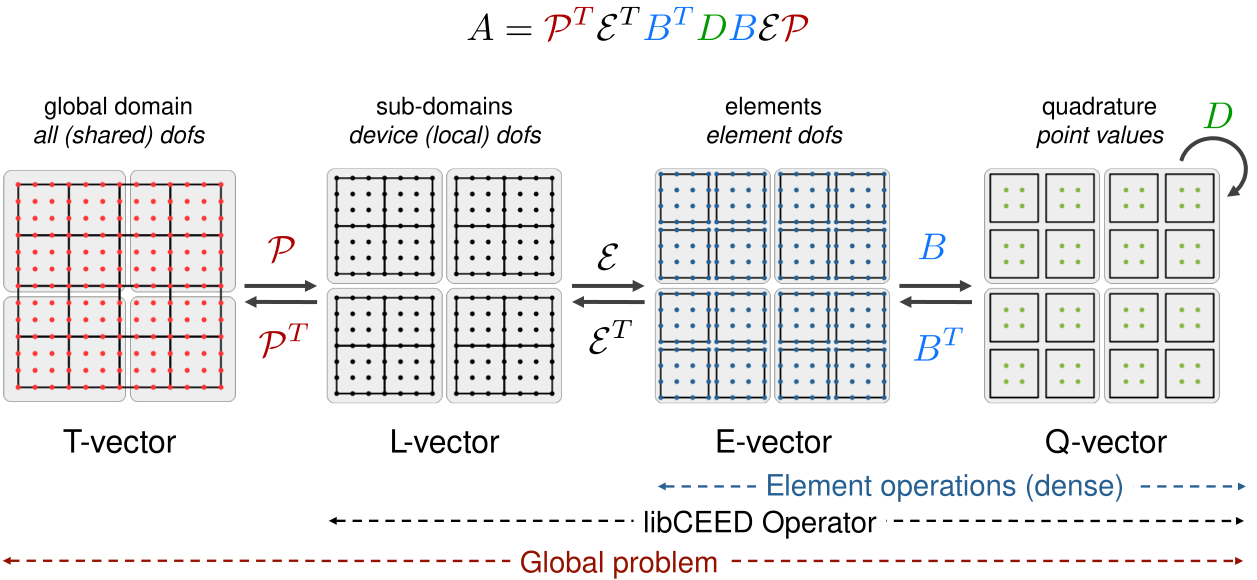
\includegraphics[height=5.0cm]{libCEEDAPI.png}

~\\

AD can be implemented in {\color{applegreen}$D$}

\end{center}
\end{frame}

%------------------------------------------------

\begin{frame}
\begin{center}
\frametitle{Enzyme AD}


\includegraphics[height=2cm]{EnzymeAD.png}

~\\

\begin{itemize}

\item Computes gradients of source code\\

~\\

\item Uses optimized LLVM IR\\

~\\

\item Performance similar to hand derivatives w/o algebraic simplification*\\

\end{itemize}

~\\

(See dissertation of Layla Ghaffari, recent PhD graduate)

\end{center}
\end{frame}

%------------------------------------------------

\begin{frame}[fragile]
\begin{center}
\frametitle{Enzyme Neo-Hookean Elasticity}

{\tiny
\begin{lstlisting}[style=boxedC]
CEED_QFUNCTION_HELPER void RatelKirchhofftau_sym_NeoHookean_AD(const CeedScalar lambda, const CeedScalar mu, CeedScalar e_sym[6], CeedScalar tau_sym[6]) {
  CeedScalar dPsi_sym[6] = {0.}, b_sym[6], dPsi[3][3], b[3][3], tau[3][3];

  // dPsi / de
  __enzyme_autodiff((void *)RatelStrainEnergy_NeoHookeanCurrentAD_Enzyme, e_sym, dPsi_sym, enzyme_const, lambda, enzyme_const, mu);
  for (CeedInt i = 3; i < 6; i++) dPsi_sym[i] /= 2.;

  // b = 2 e + I
  for (CeedInt j = 0; j < 6; j++) b_sym[j] = 2 * e_sym[j] + (j < 3);

  // tau = (dPsi / de) b
  RatelSymmetricMatUnpack(dPsi_sym, dPsi);
  RatelSymmetricMatUnpack(b_sym, b);
  RatelMatMatMult(1., dPsi, b, tau);
  RatelSymmetricMatPack(tau, tau_sym);
}

CEED_QFUNCTION_HELPER void Rateldtau_fwd(const CeedScalar lambda, const CeedScalar mu, CeedScalar e_sym[6], CeedScalar de_sym[6], CeedScalar tau_sym[6], CeedScalar dtau_sym[6]) {
  __enzyme_fwddiff((void *)RatelKirchhofftau_sym_NeoHookean_AD, enzyme_const, lambda, enzyme_const, mu, e_sym, de_sym, tau_sym, dtau_sym);
}

\end{lstlisting}
}

Enzyme computing Jacobian from Residual, via energy\\

\end{center}
\end{frame}

%------------------------------------------------

\begin{frame}
\begin{center}
\frametitle{Better Enzyme AD}


\includegraphics[height=2cm]{Rust.png} \hspace*{1cm} 
\includegraphics[height=2cm]{EnzymeAD.png}

~\\

\begin{itemize}

\item Enzyme AD available in Rust\\

~\\

\item Simplifies user experience, route to easier GPU impl\\

~\\

\item Goal of similar perf to hand derivatives of {\color{applegreen}$D$} in C\\

~\\

\item \href{https://github.com/EnzymeAD/rust}{https://github.com/EnzymeAD/rust}\\

\end{itemize}

\end{center}
\end{frame}

%-------------------------------------------------------------------------------
\section{Contact and MPM}
%-------------------------------------------------------------------------------

\begin{frame}
\begin{center}
\frametitle{Contact Models}

Nitsche method with rigid platens\\

~\\

\begin{itemize}

\item Support both Nitsche and penalty method\\

~\\

\item Contact shape either platen or cylinder\\

~\\

\item Support time dependent translation of surface\\

~\\

\item Coulomb or Threlfall friction\\

~\\

\item Deformable mesh-to-mesh contact in progress\\

\end{itemize}

~\\

(Zach R. Atkins, PhD student)

\end{center}
\end{frame}

%------------------------------------------------

\begin{frame}
\begin{center}
\frametitle{What is MPM?}

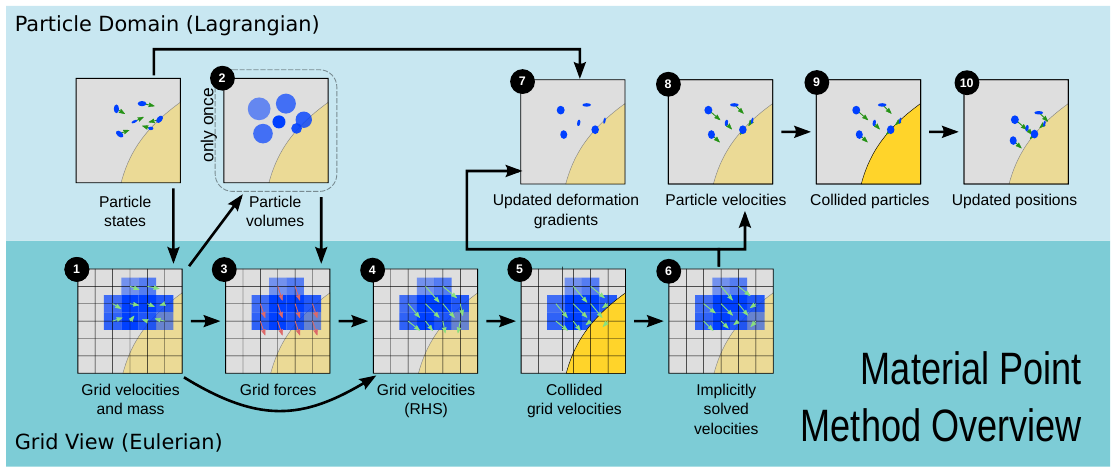
\includegraphics[height=5cm]{MPMOverview.png}\\

~\\

\begin{itemize}

\item Continuum based particle method with background mesh for gradients\\

\item Extension of FLIP (which is an extension of PIC)\\

\item Used in rendering for the movie \emph{Frozen}\\

\end{itemize}

\end{center}
\end{frame}

%------------------------------------------------

\begin{frame}
\begin{center}
\frametitle{MPM vs FEM}

MPM can be formulated as very similar to FEM\\

~\\

\begin{itemize}

\item Problem on background mesh changes when material points move\\

~\\

\item Can be viewed as FEM with arbitrary quadrature point locations\\

~\\

\item Natural fit for libCEED matrix-free representation\\

~\\

\item Ratel FEM infrastructure provides fast background mesh solves\\

\end{itemize}

~\\

(Zach R. Atkins, PhD student)

\end{center}
\end{frame}

%------------------------------------------------

\begin{frame}
\begin{center}
\frametitle{DMSwarm for Material Points}

\begin{center}
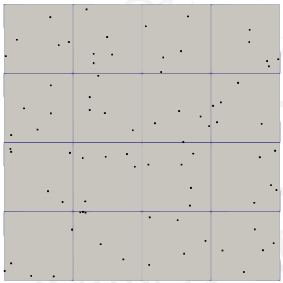
\includegraphics[height=4cm]{DMSwarmOverview.png}
\end{center}

\begin{itemize}

\item PETSc DMSwarm manages material points\\

~\\

\item Point migration on CPU only (Toulumne/El Capitan helps here!)\\

~\\

\item PETSc DMPlex manages background mesh\\

\end{itemize}

\end{center}
\end{frame}

%------------------------------------------------

\begin{frame}
\begin{center}
\frametitle{libCEED Basis Evaluation to Points}

\begin{center}
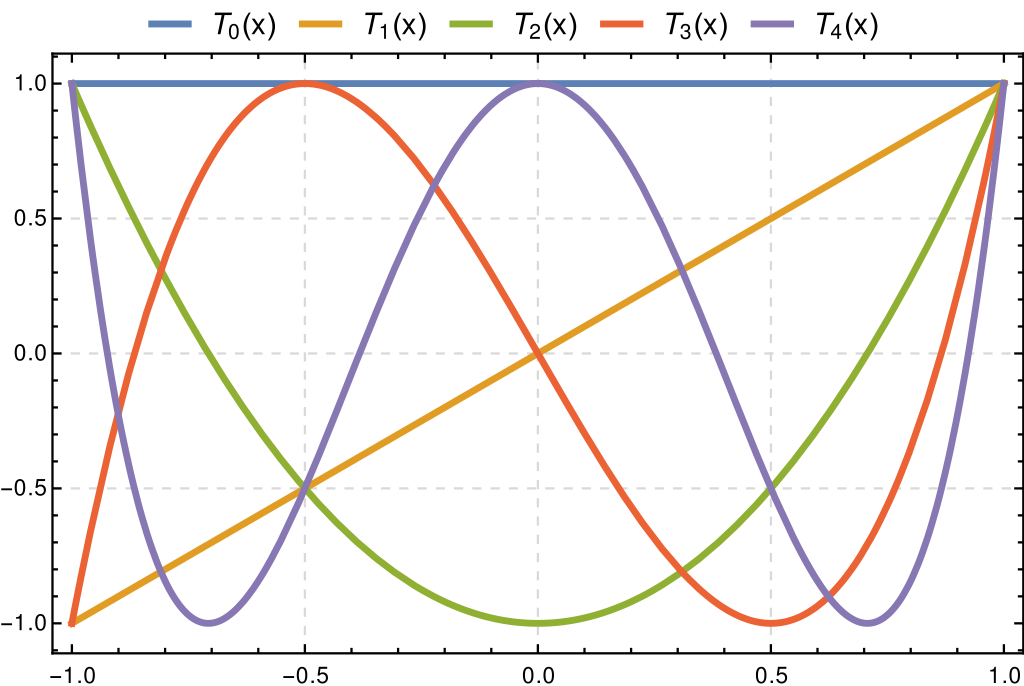
\includegraphics[height=4cm]{ChebyshevPolynomials.png}
\end{center}

\begin{itemize}

\item Interpolate from primal to dual (quadrature) space\\

~\\

\item Fit Chebyshev polynomials to values at quadrature points\\

~\\

\item Evaluate Chebyshev polynomials at arbitrary points\\

\end{itemize}

\end{center}
\end{frame}

%------------------------------------------------

\begin{frame}
\begin{center}
\frametitle{libCEED Basis Evaluation to Points}

Interpolation to Chebyshev has same FLOPs as FEM $\mathcal{O} \left( q^4 \right)$

~\\

\begin{itemize}

\item Invert map $C^{-1}$ from quadrature points to Chebyshev coeffs\\

~\\

\item Create 1D interpolation matrix $B = C N$\\

~\\

\item Tensor product: $B = \left( C \otimes C \otimes C \right) \left( N \otimes N \otimes N \right) = \left( C N \right) \otimes \left( C N \right) \otimes \left( C N \right)$\\

~\\

\item Additional cost from evaluation to arbitrary points\\

\end{itemize}

\end{center}
\end{frame}

%------------------------------------------------

\begin{frame}
\begin{center}
\frametitle{libCEED Basis Evaluation to Points}

Per point evaluation is expensive $\mathcal{O} \left( q^3 \right)$

~\\

\begin{itemize}

\item Recurrence for Chebyshev values at point\\

$f_0 = 1$, $f_1 = 2 x$, $f_n = 2 x f_{n - 1} - f_{n - 2}$\\

$f'_0 = 0$, $f'_1 = 2$, \hspace{0.7mm} $f'_n = 2 x f'_{n - 1} + 2 f_{n - 1} - f'_{n - 2}$\\

~\\

\item Contract pencil of values with element coefficients\\

~\\

\item Evaluation is independent per material point\\

~\\

\item $\mathcal{O} \left( q^3 \right)$ FLOPs at $\mathcal{O} \left( \hat{q}^3 \right)$ points\\

~\\

\item Using $p = q$, $\hat{q} = q + 1$ in current work\\

\end{itemize}

\end{center}
\end{frame}

%------------------------------------------------

\begin{frame}[fragile]
\begin{center}
\frametitle{Example - MPM Sinker}

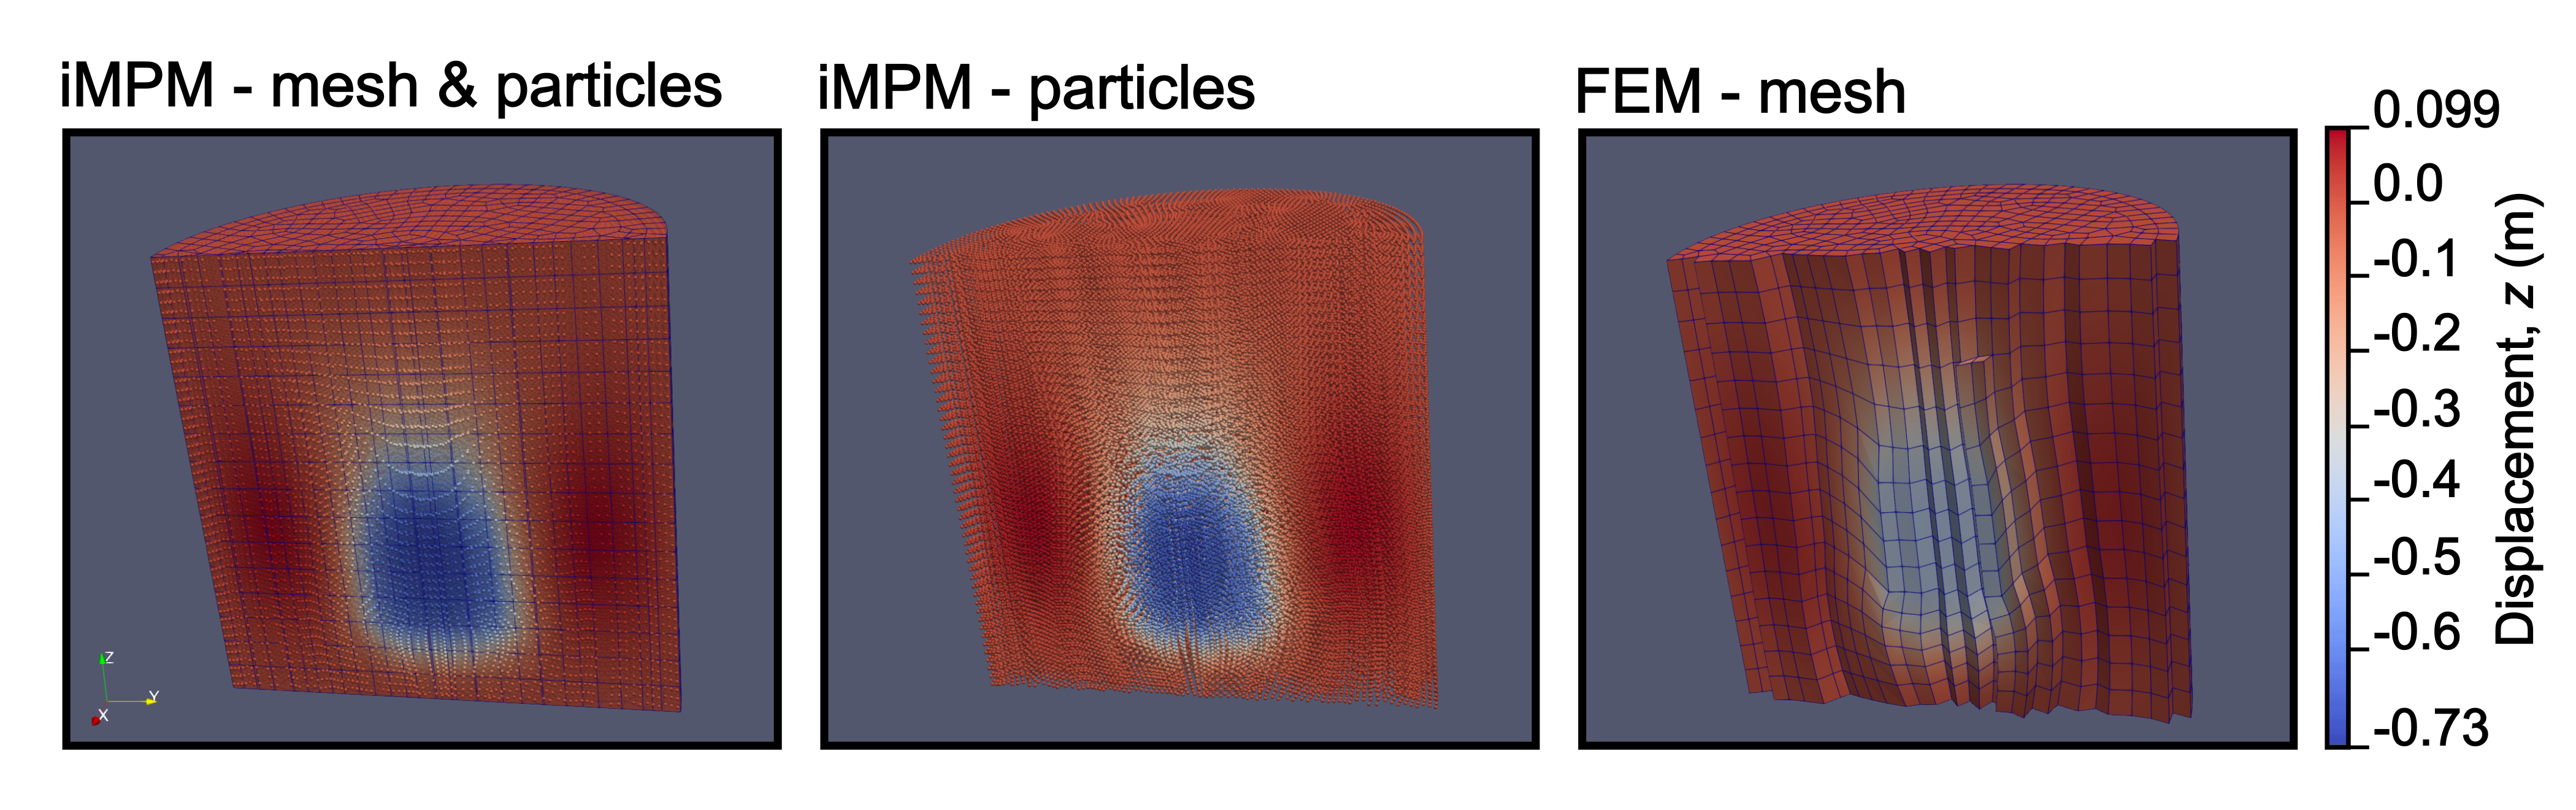
\includegraphics[height=3.8cm]{sinker-MPM-FEM.png}

{\tiny
\begin{lstlisting}
$ bin/ratel-quasistatic -options_file examples/ymls/ex02-quasistatic-elasticity-mpm-neo-hookean-damage-current-sinker-cylinder.yml
\end{lstlisting}
}

FEM, iMPM simulations of dense sinker in "foam" validation problem\\

(Mesh distortion limits FEM simulation)

\end{center}
\end{frame}

%------------------------------------------------

\begin{frame}
\begin{center}
\frametitle{Example - Press Simulation}

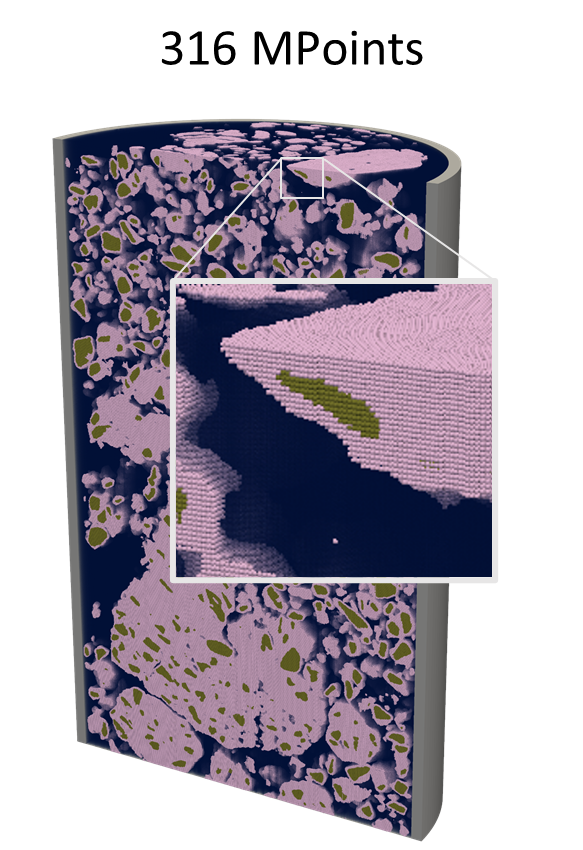
\includegraphics[height=5cm]{iMPMCloseup.png}
\hspace*{1cm}
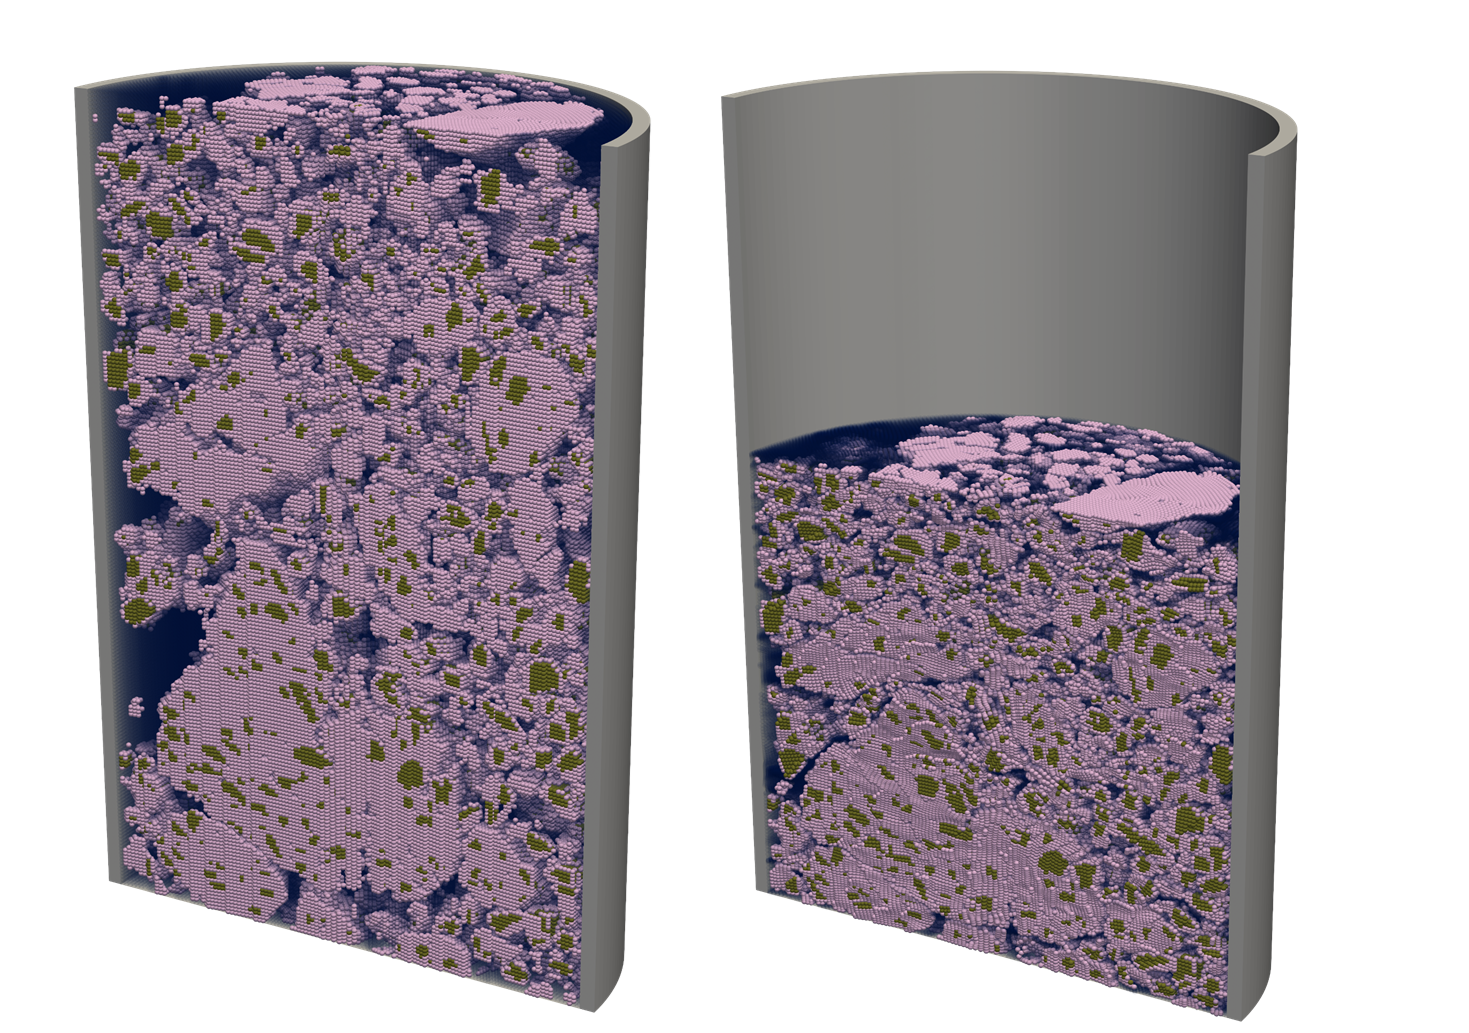
\includegraphics[height=5cm]{iMPMCompress.png}

~\\

Compression of mock HE grains (gold) and binder (pink) mixture\\

(Reset background mesh to computational region on each timestep)

\end{center}
\end{frame}

%------------------------------------------------

\begin{frame}
\begin{center}
\frametitle{Ratel PCpMG}

pMG giving promising initial results with GPU impl\\

~\\

\begin{itemize}

\item Neo-Hookean finite strain elasticity with damage\\

~\\

\item Confined press of grain/binder with "sticky air" voids\\

~\\

\item Jacobi iterations tend to double with 2x refinement\\

~\\

\item pMG iteration counts robust with refinement\\

\end{itemize}

\begin{table}[ht!]
\begin{center}
\begin{tabular}{l r r r}
  \toprule
             & Material Points & Jacobi its & pMG its  \\
  \toprule
  Coarse     &         388,800 &   900-1000 &   35-45  \\
  Fine       &       7,372,800 &      -     &   25-40  \\
  \bottomrule
\end{tabular}
\end{center}
\end{table}

\end{center}
\end{frame}

%-------------------------------------------------------------------------------
\section{Questions}
%-------------------------------------------------------------------------------

\begin{frame}
\frametitle{Questions?}

\begin{center}
\includegraphics[height=2.75cm]{libCEEDlogo.png}
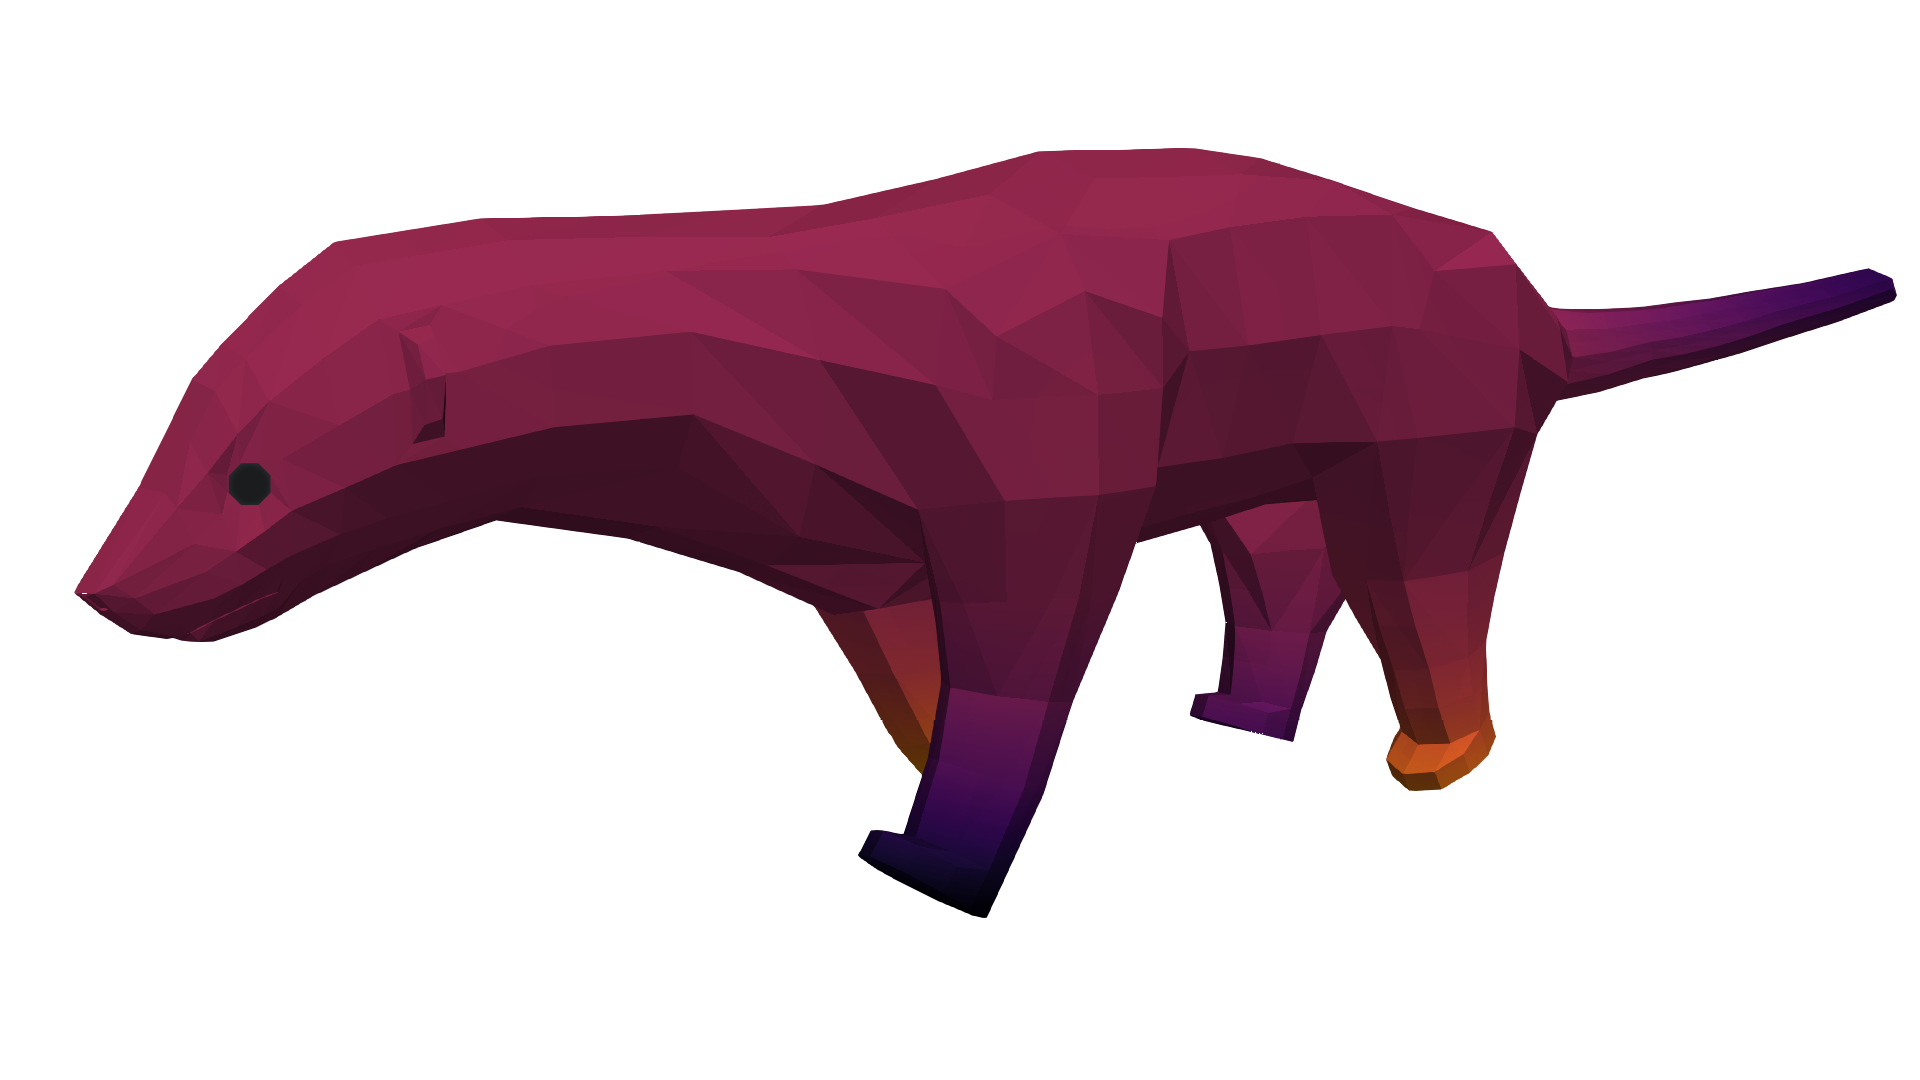
\includegraphics[height=2.75cm]{Ratellogo.png}
\end{center}

{\flushleft

libCEED Repo: \href{https://github.com/CEED/libCEED}{https://github.com/CEED/libCEED}\\
Ratel Repo: \hspace*{0.39cm} \href{https://gitlab.com/micromorph/ratel}{https://gitlab.com/micromorph/ratel}\\

~\\

Grant: Predictive Science Academic Alliance Program (DE-NA0003962)\\

}

\begin{center}

\includegraphics[height=0.8cm]{psaap-center-logos.png}
\end{center}

\end{frame}

%-------------------------------------------------------------------------------

\begin{frame}[noframenumbering]
\titlepage % Print the title page
\end{frame}

%-------------------------------------------------------------------------------

\end{document}

%-------------------------------------------------------------------------------
